%% AIAA Journal submission. Uses the AIAA class `new-aiaa` (Overleaf), journal format:
%% single-column, double-spaced, 10pt Times. Requires new-aiaa.cls + new-aiaa.bst (this directory)
%% and the newtx fonts. Build: pdflatex main; bibtex main; pdflatex main; pdflatex main.
\documentclass[journal]{new-aiaa}

\usepackage{graphicx}
\usepackage{float}
\usepackage{amsmath}
\usepackage{booktabs}

\renewcommand{\topfraction}{0.9}
\renewcommand{\bottomfraction}{0.8}
\renewcommand{\textfraction}{0.07}
\renewcommand{\floatpagefraction}{0.8}

\graphicspath{{figs/}}

\title{A Single-Equation Transition Model: The Spalart--Allmaras Working
Variable as an Amplification Factor}

\author[1,2]{Qiqi Wang\footnote{Founding Technologist, Flexcompute, Inc.;
Associate Professor, Department of Aeronautics and Astronautics, Massachusetts
Institute of Technology. AIAA Associate Fellow.}}
\affil[1]{Flexcompute, Inc.}
\affil[2]{Department of Aeronautics and Astronautics, Massachusetts Institute of Technology}

\begin{document}
\maketitle

\begin{abstract}
Conventional Reynolds-averaged Navier--Stokes (RANS) transition models add a
transport equation for an auxiliary variable (amplification factor,
intermittency, or transition Reynolds number) or gate turbulent production with
an algebraic intermittency. The Spalart--Allmaras (SA) working variable
$\tilde\nu$ already spans laminar to fully turbulent values; its sub-$O(\nu)$
range, inert in the baseline model, carries a Tollmien--Schlichting amplification
factor. A single modified production term drives the same transport equation
through laminar instability growth and turbulent eddy-viscosity production,
handing over near $\chi\!=\!\tilde\nu/\nu\!\sim\!1$; no auxiliary field is
introduced. The amplification rate depends only on the local mean flow---a
vorticity Reynolds number and a profile-fullness indicator---so the production
retains an analytic Jacobian and integrates implicitly at the cost of the
baseline model. On flat plates the model recovers the laminar and turbulent
skin-friction laws with a transition between them. On a NACA~0012 at $Re=10^6$
and $\alpha=0^\circ$ it gives a half-chord laminar run and a $\sim\!31\%$ drag
reduction, agreeing to $0.5\%$ across a structured O-grid and an anisotropic
unstructured mesh---a reduction unreachable by fully turbulent SA. Across
$-2^\circ\!\le\!\alpha\!\le\!8^\circ$ on the NACA~0012 and an NLF(1)-0416, the
predicted transition tracks an $e^N$ reference on both grids and recovers the
NLF drag bucket.
\end{abstract}

\section*{Nomenclature}
\begin{tabbing}
  $N,\;N_\mathrm{crit}$\quad\quad \= \kill
  $\tilde\nu$ \> SA working variable \\
  $\nu$ \> kinematic (laminar) viscosity \\
  $\chi$ \> $\tilde\nu/\nu$ \\
  $d$ \> distance to the nearest wall \\
  $\omega$ \> vorticity magnitude \\
  $Re_\Omega$ \> vorticity Reynolds number, $d^2\omega/\nu$ \\
  $\Gamma$ \> velocity-profile fullness indicator, Eq.~\eqref{eq:indicators} \\
  $\sigma_t$ \> laminar-to-turbulent handover weight \\
  $P,\;D$ \> production and destruction of $\tilde\nu$ \\
  $N,\;N_\mathrm{crit}$ \> amplification factor and its critical value ($e^N$ method) \\
  $Tu$ \> freestream turbulence intensity \\
  $\chi_\infty$ \> freestream value of $\chi$ \\
  $C_f,\;C_D,\;C_L$ \> skin-friction, drag, and lift coefficients \\
  $Re_x,\;Re_\theta$ \> streamwise and momentum-thickness Reynolds numbers \\
  $c_{\nu,\mathrm{aft}}$ \> laminar-viscosity scale factor in the SA cross-stream diffusion only ($1/12$) \\
\end{tabbing}

\section{Introduction}

Laminar flow over a lifting surface offers among the largest viscous-drag
reductions available, and predicting where it ends is a first-order requirement
for natural-laminar-flow design.
In a quiet low-disturbance environment the laminar boundary layer first becomes
unstable to gentle two-dimensional Tollmien--Schlichting (TS) waves
\cite{mack_1977,schmid_henningson_2001}: as the layer thickens, the envelope of the
strongest TS mode grows quasi-exponentially over a long streamwise stretch until,
at an amplitude of a few percent of the mean, three-dimensional secondary
instabilities trigger localized turbulent spots that spread and merge into a fully
turbulent layer \cite{schubauer_klebanoff_1956,schmid_henningson_2001}. The slow
TS-envelope stage occupies most of the streamwise distance and largely determines
where transition is observed, so it is the stage a transition model must reproduce.
The classical tool is the $e^N$ method \cite{smith_gamberoni_1956, vaningen_2008}:
linear stability theory is integrated along the boundary layer to accumulate an
amplification factor $N$, and transition is declared where $N$ reaches an empirical
threshold $N_\mathrm{crit}$ set by the disturbance environment \cite{mack_1977}.
Drela and Giles reduced the stability integration to an approximate envelope
correlation, making $e^N$ practical inside an integral-boundary-layer method
\cite{drela_giles_1987, drela_xfoil_1989}.

The $e^N$ method is non-local: it presumes a boundary layer that can be marched and
integrated, which is foreign to a general unstructured RANS solver. The community
has therefore recast transition in terms of locally computable transport equations,
along three lines. \emph{Amplification factor transport} carries $N$ itself: Coder
and Maughmer's AFT model transports an amplification factor whose source reproduces
the $e^N$ envelope and couples it to SA through the $f_{t2}$ term, the variant
catalogued as SA-AFT2017b on the NASA Turbulence Modeling Resource adding a second
(intermittency) equation \cite{coder_maughmer_2014, nasa_tmr}; Halila et al.
subsequently smoothed this model (AFT-S) for implicit Newton--Krylov solution in
gradient-based optimization, retaining the separate amplification-factor equation
\cite{halila_2022}. \emph{Local-correlation intermittency transport} instead carries
an intermittency: the Langtry--Menter $\gamma$--$Re_\theta$ model adds two transport
equations \cite{menter_langtry_2006, langtry_menter_2009}, reduced to one in a later
$\gamma$-only formulation \cite{menter_gamma_2015} and coupled to SA by Medida and
Baeder \cite{medida_baeder_2011}; Walters and Cokljat instead transport a
laminar-fluctuation energy \cite{walters_cokljat_2008}. Finally, \emph{algebraic}
models add no transport equation at all: the Bas--Cakmakcioglu model and its
revision (BC/BCM) multiply the SA production by an intermittency computed from
purely local correlations \cite{cakmakcioglu_2018, cakmakcioglu_2020}, an approach
extended in several recent SA modifications \cite{rahman_2024, crivellini_2023}.

These nearest neighbors share a common premise that we depart from: the SA working
variable $\tilde\nu$ is treated as a purely turbulent quantity, switched on either
by an extra transported field (AFT, $\gamma$--$Re_\theta$) or by an external
algebraic intermittency (BC/BCM). Equation count alone therefore does not separate
the present approach from the algebraic family, which is also single-equation. The
distinction is in \emph{what the field represents}. A scaling argument shows the
sub-$O(1)$ range of $\tilde\nu$ is the natural home for a TS-envelope variable. The SA working variable carries the dimensions of an eddy viscosity, i.e.\
a product $u'\ell$ of a fluctuation-velocity scale and a length scale. In a
Blasius-like layer just before secondary instability, the TS-envelope velocity
amplitude is a few percent of the mean and the coherent structures are confined to a
fraction of the boundary-layer thickness at
$Re_\theta\!\sim\!\mathcal{O}(10^2)$--$\mathcal{O}(10^3)$
\cite{schmid_henningson_2001,abu_ghannam_shaw_1980}; the product is at most a few
times the laminar viscosity $\nu$, i.e.\ $\chi=\tilde\nu/\nu\!\lesssim\!\mathcal{O}(1)$.
The region $\chi\!\lesssim\!\mathcal{O}(1)$ is exactly the part of the SA state space
that contributes negligibly to the eddy viscosity and is largely inert in the
baseline model \cite{spalart_allmaras_1994}. The natural amplitude and length scales
of laminar instabilities therefore correspond to a range of $\tilde\nu$ that SA
barely uses---a coincidence we exploit: we let that range \emph{be} the amplification
factor. In the laminar regime the production of $\tilde\nu$ is replaced by a local,
envelope-method-inspired instability rate, so $\ln\tilde\nu$ accumulates
monotonically in the manner of an amplification factor; as $\tilde\nu$ approaches its
turbulent level the production reverts smoothly to the standard SA form. One
transport equation---the SA equation, unchanged in structure---spans laminar
instability and turbulence with no auxiliary field. We refer to the model as SA-AF
(the SA working variable serving as the \emph{a}mplification \emph{f}actor); it is
distinct from Coder's SA-AFT, in which a separate amplification factor is
transported.

The contribution is thus a model that occupies an otherwise empty cell
(Table~\ref{tab:taxonomy}): amplification-factor ($e^N$-like) physics carried by the
turbulence working variable itself, with no auxiliary equation and a local,
analytically differentiable source.

\begin{table}[t]
  \centering
  \caption{RANS-compatible transition-model families and where the present model
  (SA-AF) sits. ``Extra equations'' counts transport equations beyond the baseline
  turbulence model.}
  \label{tab:taxonomy}
  \begin{tabular}{lcl}
    \toprule
    Family & Extra eqns & Transition mechanism \\
    \midrule
    $e^N$ envelope \cite{smith_gamberoni_1956, drela_giles_1987} & --- (non-local) & stability-integral $N$ \\
    AFT \cite{coder_maughmer_2014, halila_2022} & $1$--$2$ & transported amplification factor \\
    $\gamma$--$Re_\theta$ \cite{langtry_menter_2009, medida_baeder_2011} & $2$ & transported intermittency, $Re_{\theta t}$ \\
    one-equation $\gamma$ \cite{menter_gamma_2015} & $1$ & transported intermittency \\
    algebraic SA \cite{cakmakcioglu_2018, rahman_2024} & $0$ & local intermittency gates production \\
    \textbf{SA-AF (present)} & $\mathbf{0}$ & working variable \emph{is} the factor \\
    \bottomrule
  \end{tabular}
\end{table}
SA-AF is scoped to natural (Tollmien--Schlichting) transition. A single
calibration of the local amplification rate (one sigmoid kernel
$a(\Gamma)$ pinned at two physical anchors --- a flat-plate amplification
rate set by matching Schubauer--Skramstad transition Reynolds numbers, and
an adverse-pressure-gradient saturation rate set by an NLF airfoil
case) is used unchanged for the Blasius transport verification and for
all coupled-RANS computations on flat plate and airfoil.
Sections~\ref{sec:flatplate} and \ref{sec:airfoil} verify it on a flat plate
and validate it on a NACA~0012 in a production RANS solver.

\section{Model Formulation}\label{sec:model}

The Spalart--Allmaras model \cite{spalart_allmaras_1992} solves a transport equation
for $\tilde\nu$,
\begin{equation}
  \frac{D\tilde\nu}{Dt} = P_\mathrm{SA} - D_\mathrm{SA}
  + \frac{1}{\sigma}\nabla\!\cdot\!\big[(\nu+\tilde\nu)\nabla\tilde\nu\big]
  + \frac{c_{b2}}{\sigma}|\nabla\tilde\nu|^2,
  \qquad
  P_\mathrm{SA} = c_{b1}\tilde S\,\tilde\nu,
  \quad
  D_\mathrm{SA} = c_{w1}f_w\!\left(\frac{\tilde\nu}{d}\right)^{\!2},
  \label{eq:sa}
\end{equation}
in the standard form of Ref.~\cite{spalart_allmaras_1992}, with the modified
vorticity $\tilde S$, the wall function $f_w$, the constants $c_{b1},c_{b2},c_{w1},
\sigma$, and the eddy viscosity $\mu_t=\rho\,\tilde\nu f_{v1}(\chi)$,
$\chi=\tilde\nu/\nu$, all as defined there; we use the negative-$\tilde\nu$
safeguards of the standard implementation. Because $f_{v1}\!\to\!0$ as
$\chi\!\to\!0$, the field $\tilde\nu$ contributes negligibly to the mean flow while
$\chi\lesssim1$: this sub-$O(1)$ range is dynamically inert in the baseline model
and is what we repurpose.

\subsection{Laminar amplification production}
In a laminar boundary layer we replace the SA production by a local instability rate
of the kind used in approximate-envelope $e^N$ methods. The envelope $e^N$ rate
$dN/dRe_\theta$ is naturally written in terms of the integral
momentum thickness $\theta$, but $\theta$ is awkward to evaluate in a general RANS
field because it requires integration ``to the edge'' of a boundary layer whose edge
may be ill-defined under shear-layer merging, separation, or freestream turbulence.
A clean local surrogate is the vorticity Reynolds number
$Re_\Omega=d^2\omega/\nu$ \cite{VanDriest1963, MenterLangtry2006, langtry_menter_2009}:
in a Blasius boundary layer the peak of $Re_\Omega$ inside the BL profile is
proportional to $Re_\theta$ ($\max_y Re_\Omega\!\approx\!2.2\,Re_\theta$) and is
located at $y\!\approx\!\theta$, so $Re_\Omega$ inherits the role of $Re_\theta$
without the nonlocal integration (Fig.~\ref{fig:amp}). We adopt $Re_\Omega$ as the
amplification indicator and pair it with a profile-fullness indicator
\begin{equation}
  Re_\Omega = \frac{d^2\,\omega}{\nu}, \qquad
  \Gamma = \frac{2(\omega d)^2}{|\mathbf{u}|^2+(\omega d)^2},
  \label{eq:indicators}
\end{equation}
where $\Gamma\in[0,2]$ approaches unity in a near-wall shear layer (where
$\omega d\!\sim\!|\mathbf{u}|$) and grows toward 2 on an inflectional profile.
$\Gamma$ is a local surrogate for the role played by the shape factor in envelope
methods and is not the boundary-layer shape factor $H$ itself.

The velocity magnitude $|\mathbf{u}|$ in Eq.~\eqref{eq:indicators} is the flow
speed measured relative to the nearest wall point. Because that reference is
fixed to the body, $|\mathbf{u}|$ is Galilean invariant, as are $\omega$ and $d$:
a uniform frame translation moves flow and wall point together. The indicators
\eqref{eq:indicators} thus inherit the locality and frame independence of the
wall-distance dependence already built into the baseline SA model, and require
no nonlocal integration.

The non-dimensional amplification rate is a smooth sigmoid in $\Gamma$
gated below a vorticity-Reynolds floor $Re_\Omega^{\mathrm{f}}$,
\begin{equation}
  a(Re_\Omega,\Gamma) = a_{\max}\,S\!\big(z\big),\quad
  z = s\,(\Gamma - g_c)
      + \ln\!\Big(1-\big(\tfrac{Re_\Omega^{\mathrm{f}}}{Re_\Omega}\big)^{p}\Big),\quad
  S(z)=\frac{1}{1+e^{-z}},
  \label{eq:rate}
\end{equation}
with $a\equiv0$ for $Re_\Omega\le Re_\Omega^{\mathrm{f}}$. The floor
$Re_\Omega^{\mathrm{f}}\!=\!100$ is chosen so the Blasius growth onset
matches Drela's $Re_{\theta,\mathrm{crit}}\!\approx\!200$ for the
zero-pressure-gradient profile. The barrier is $\Gamma$-independent:
favorable-pressure-gradient suppression is handled separately by a streamwise
pressure-gradient sensor (see below), avoiding the contamination of Blasius
growth that a $\Gamma$-dependent (slanted) cliff would otherwise cause. The second term in $z$ is the
log barrier centered on this cliff: it drives $z\!\to\!-\infty$ as
$Re_\Omega\!\to\!Re_\Omega^{\mathrm{c}}(\Gamma)^{+}$ and vanishes very rapidly
for $Re_\Omega\!>\!Re_\Omega^{\mathrm{c}}$ (the high exponent $p\!=\!4$ makes
the barrier sharply local to the cliff, so $1\!-\!(Re_\Omega^{\mathrm{c}}/
Re_\Omega)^p\!\approx\!1$ once $Re_\Omega\!\gtrsim\!2\,Re_\Omega^{\mathrm{c}}$).
This preserves the calibrated band away from the cliff while delivering a
hard cutoff at it.
It enforces both the sublayer cutoff ($\Gamma\!\to\!1$ near the wall is a
generic asymptote rather than a true instability) and the favorable-PG
suppression (where $\Gamma_{\max}$ still sits at the wall asymptote
$\Gamma\!=\!1$ but $Re_\Omega$ is too low to be linearly unstable); the
exponent $p\!=\!4$ gives a sharp drop to zero at the cliff (a near-Heaviside
cutoff) while leaving $Re_\Omega\!\gtrsim\!2\,Re_\Omega^{\mathrm{c}}$
essentially unattenuated. Because
$Re_\Omega\!=\!d^2\omega/\nu\!\to\!0$ at the wall, this barrier suppresses the
viscous sublayer robustly under mesh refinement. The rate \eqref{eq:rate}
remains independent of $\tilde\nu$, so the implicit Jacobian below is
unchanged.

The laminar production is
\begin{equation}
  P_\mathrm{AFT} = a(Re_\Omega,\Gamma,\lambda_p)\,\omega\,\tilde\nu ,
  \label{eq:paft}
\end{equation}
where the rate carries an additional dependence on the local streamwise
pressure-gradient sensor $\lambda_p$ (defined below) that suppresses
favorable-pressure-gradient amplification. Specifically,
\begin{equation}
  a(Re_\Omega,\Gamma,\lambda_p) =
       a_{\max}\,\sigma_\Gamma\!(s(\Gamma-g_c))\cdot
       \big[1-(Re_\Omega^{\mathrm{f}}/Re_\Omega)^p\big]\cdot
       \sigma_\mathrm{FPG}(\lambda_p),
  \label{eq:rate_with_fpg}
\end{equation}
with the same $\Gamma$-sigmoid and cliff floor as before, and the new
favorable-pressure-gradient suppression
\begin{equation}
  \sigma_\mathrm{FPG}(\lambda_p) =
       \frac{1}{1+\exp(s_\lambda(\lambda_p-\lambda_\ast))},
  \qquad
  \lambda_p = -\,\frac{d^{2}}{\rho\,\nu\,|\mathbf{u}|^{2}}\,\mathbf{u}\cdot\nabla p .
  \label{eq:fpg}
\end{equation}
$\lambda_p$ is a purely local Pohlhausen-like indicator: it is positive
where the flow is accelerating (favorable PG, $\partial p/\partial s\!<\!0$),
zero on a zero-pressure-gradient (Blasius) profile, and negative under
adverse PG. Calibrated against Falkner--Skan profiles at $\eta\!\approx\!1$
(the kernel-active band): Blasius gives $\lambda_p\!=\!0$, Hiemenz
($\beta\!=\!1$) gives $\lambda_p\!\approx\!1.29$. Anchors
$\sigma_\mathrm{FPG}(0)\!=\!0.95$ and $\sigma_\mathrm{FPG}(1.29)\!=\!0.05$
yield $(\lambda_\ast, s_\lambda) = (0.64, 4.56)$. Adverse PG ($\lambda_p\!<\!0$)
sees $\sigma_\mathrm{FPG}\!>\!0.95$, leaving the inflectional-profile
amplification (which $\Gamma$-sigmoid already captures) untouched.
$\lambda_p$ is Galilean invariant (pressure differences are frame
independent), local (no nonlocal integration), and independent of
$\tilde\nu$, so it preserves the analytic Jacobian of
Sec.~\ref{sec:impl}.

\paragraph{FPG-modulated cliff floor.} $\sigma_\mathrm{FPG}$ alone reduces
the growth \emph{rate} in favorable-pressure-gradient regions, but does not
delay the growth \emph{onset}. To match the airfoil rooftop start-of-growth
location, the cliff floor is also amplified by $\lambda_p$:
\begin{equation}
  Re_\Omega^{\mathrm{c}}(\lambda_p) =
        Re_\Omega^{\mathrm{f}}\,
        \exp\!\big[K_\lambda\,\max(0,\lambda_p)\big].
  \label{eq:cliff_fpg}
\end{equation}
$K_\lambda\!=\!10$ is calibrated against the NLF(1)-0416 $\alpha=0^\circ$
rooftop where mfoil's $e^N$ method puts $N\approx 0$ until $x/c\approx 0.2$.
For $\lambda_p\!\le\!0$ (zero or adverse PG), the cliff floor reverts to
$Re_\Omega^{\mathrm{f}}\!=\!100$ exactly, so Blasius and adverse-PG profiles
are unaffected.
Equation~\eqref{eq:paft} grows $\tilde\nu$ along the flow at the local rate
$a\,\omega$, so $\ln(\tilde\nu/\tilde\nu_\infty)$ accumulates monotonically in the
manner of an amplification factor $N$; because $a_{\max}$ is small
(Sec.~\ref{sec:calib}) the accumulation is gentle and is calibrated for onset
location rather than to match the $e^N$ growth rate quantitatively. Transition is
reached when $\tilde\nu$ has grown to $\chi\sim1$, where the eddy viscosity becomes
dynamically active.

\subsection{Single-equation blend}
A handover weight ties the laminar and turbulent regimes to the single state
variable through $\chi$,
\begin{equation}
  \sigma_t(\chi) = \max\!\left[\,1-e^{-(\chi-1)/\tau},\;0\right] \;=\;
  \begin{cases} 0, & \chi \le 1, \\ 1-e^{-(\chi-1)/\tau}, & \chi > 1, \end{cases}
  \label{eq:sigma}
\end{equation}
zero for $\chi\le1$ (laminar) and asymptotically approaching unity as $\chi\!\gg\!1$
(turbulent). The
production and destruction of Eq.~\eqref{eq:sa} are blended,
\begin{equation}
  P = \max\!\big[(1-\sigma_t)\,P_\mathrm{AFT},\;\sigma_t\,P_\mathrm{SA}\big], \qquad
  D = \sigma_t\,D_\mathrm{SA}.
  \label{eq:blend}
\end{equation}
The $\max$ form, rather than a convex sum, matters for one reason: it hands the
production cleanly from amplification to SA. For $\chi\le1$ ($\sigma_t=0$) it is
\emph{identical} to a convex blend, $\max[P_\mathrm{AFT},0]=P_\mathrm{AFT}$, so the
laminar amplification---and with it the entire $e^N$ calibration---is unchanged. Once
$\sigma_t P_\mathrm{SA}$ overtakes the amplification (just past $\chi=1$, since
$P_\mathrm{SA}\!\gg\!P_\mathrm{AFT}$ there) the laminar term is dropped entirely, so the
\emph{pressure-gradient-sensitive} amplification carries no weight downstream of
transition. A convex sum instead retains a $(1-\sigma_t)P_\mathrm{AFT}$ bleed through
the handover; on a fine grid resolving a marginal natural transition this residual
receptivity couples the transition location to the airfoil's global circulation and
produces a self-sustained limit cycle (Sec.~\ref{sec:blendnlf}). The $\max$ removes it and
the computation converges to a steady state. Gating destruction by $\sigma_t$ is
essential: SA destruction is a turbulent wall-damping term that would suppress
the gentle laminar amplification. The limit $\sigma_t\!\to\!1$ recovers the unmodified SA equation
\emph{exactly}, so the fully turbulent calibration (log law, freestream decay) is
preserved; in the laminar range the equation is a pure
advection--diffusion--amplification balance for $\tilde\nu$.
The diffusion terms of Eq.~\eqref{eq:sa} are retained throughout and provide the
cross-stream smoothing of the disturbance envelope, with one adjustment: the
laminar coefficient in the SA cross-stream diffusion is scaled by
$c_{\nu,\mathrm{aft}}\!=\!1/12$,
$(\nu+\tilde\nu)\!\to\!(c_{\nu,\mathrm{aft}}\nu+\tilde\nu)$ in the diffusion
term of Eq.~\eqref{eq:sa}. The mean-flow viscosity and the SA destruction are
untouched. The reduced cross-stream smearing keeps the in-BL $\tilde\nu$ peak
co-located with the $Re_\Omega$ peak and recovers a $dN/dRe_\theta$ growth rate
in the Drela envelope range; setting $c_{\nu,\mathrm{aft}}\!=\!1$ broadens the
peak and roughly halves the effective amplification.

\subsection{Implicit integrability}
The amplification rate \eqref{eq:rate} depends only on the local mean flow
($\omega$, $\mathbf{u}$, $d$, $\nu$) and not on $\tilde\nu$. Within a segregated
turbulence solve, in which the mean-flow state is frozen over a turbulence
sub-iteration, $P_\mathrm{AFT}$ is therefore strictly linear in $\tilde\nu$ and its
contribution to the implicit Jacobian is the analytic constant $a\,\omega$. The only
$\tilde\nu$-nonlinear term introduced by the blend is the smooth handover
$\sigma_t(\chi)$, whose derivative is bounded and available in closed form. The
modified source thus carries an exact analytic Jacobian and is integrated by the same
implicit, Jacobian-based scheme as the baseline model, in contrast to the difficulty
of converging a sharp transition switch; this is the same motivation that led Halila
et al. to smooth the AFT model for implicit solution \cite{halila_2022}, achieved
here without an auxiliary equation. The amplification magnitude $a_{\max}$ is kept
small so that the eddy viscosity rises gently through transition: a sharp rise
destabilizes the mean-flow coupling, and a gentle rise additionally widens the
sensitivity of the transition location to the disturbance environment.

\section{Calibration}\label{sec:calib}

The amplification rate \eqref{eq:rate} carries the global magnitude
$a_{\max}$, the $\Gamma$-sigmoid parameters $(s,g_c)$, and the cliff
parameters $(Re_\Omega^{\mathrm{f}}, \eta, p)$. We fix $(s,\,g_c)=(5.263,\,
1.572)$ structurally: $\Gamma\!=\!1$ is the wall-asymptote of $\max_y\Gamma$
in any attached zero- or favorable-pressure-gradient boundary layer (a
consequence of $\omega\,d/|V|\!\to\!1$ at the wall with monotone-decreasing
shear), so $g_c$ slightly above $1$ keeps Blasius near the sigmoid foot
while $\Gamma\!\to\!2$ on an inflectional / near-separation profile
saturates the sigmoid for adverse pressure gradients. The
$\Gamma$-independent cliff floor $Re_\Omega^{\mathrm{f}}\!=\!100$ places
Blasius growth onset at Drela's $Re_{\theta,\mathrm{crit}}\!\approx\!200$
for the zero-pressure-gradient profile. Favorable-pressure-gradient
suppression is delegated to a separate streamwise pressure-gradient sensor
(Sec.~\ref{sec:fpg}), so the cliff floor is purely a sublayer / onset cutoff
and does not need a $\Gamma$-dependent tilt that would otherwise contaminate
Blasius growth.

The remaining global magnitude $a_{\max}\!=\!0.15$ is set by matching the
model's predicted transition $Re_\theta^{\mathrm{tr}}$ to the
Schubauer--Skramstad flat-plate data \cite{schubauer_skramstad_1948} across
five freestream turbulence levels (Sec.~\ref{sec:flatplate}), jointly with
the Tu$\to\chi_\infty$ slope $B$ of Eq.~\eqref{eq:tumap}. The cliff threshold
$Re_\Omega^{\mathrm{c}}(\Gamma)$ of Eq.~\eqref{eq:cliff} suppresses growth
both near the wall (where $\Gamma\!\to\!1$ yet $Re_\Omega\!\to\!0$) and on
favorable-pressure-gradient profiles whose peak $\Gamma$ is pinned at $1$ but
whose $Re_\Omega$ is still low; envelope-style onset arises naturally once a
thicker boundary layer brings the
in-BL peak of $Re_\Omega$ into the unstable band. The constant $2.2$ relating
$\max_y Re_\Omega$ to $Re_\theta$ in a Blasius profile is what carries the
classical $\theta$-based envelope rate into the present local formulation.

Figure~\ref{fig:amp} shows that on a Blasius profile the rate $a\,\omega$ is
concentrated in a band at intermediate wall distance---the part of the profile
where Tollmien--Schlichting waves extract energy from the mean shear---and
vanishes in the viscous sublayer and the outer flow, in the manner of the local
growth rate of envelope $e^N$ methods. Taking the peak of the local kernel
across the wall-normal direction and converting from $x$ to $Re_\theta$ recovers
an envelope rate of a flat plate (Fig.~\ref{fig:amp}, right) that rises
monotonically with $Re_\theta$ through the unstable range, in the range of
Drela-style envelope-$e^N$ rates at the calibrated intensity
$a_{\max}\!=\!0.2$.

To confirm that the working variable, in its sub-$O(1)$ range, behaves as an
amplification factor, we solve the disturbance transport equation in non-dimensional
boundary-layer variables (length in $\nu/U_\infty$, velocities normalized by
$U_\infty$),
\begin{equation}
  u\,\frac{\partial\hat\nu}{\partial x} + v\,\frac{\partial\hat\nu}{\partial y}
  = \frac{1}{\sigma_\mathrm{SA}}\,\frac{\partial^2\hat\nu}{\partial y^2}
    + a(Re_\Omega,\Gamma)\,\omega\,\hat\nu,
  \label{eq:transport}
\end{equation}
with the SA cross-stream diffusion coefficient $\sigma_\mathrm{SA}\!=\!2/3$ retained
from the laminar limit of the SA equation.
on the Blasius layer, seeded with $\hat\nu_\infty=1$ at the leading edge as a
unit-scale reference, so that $N\!=\!\ln(\hat\nu/\hat\nu_\infty)\!=\!\ln\hat\nu$ is the
amplification factor by construction. Figure~\ref{fig:nuhat} shows
$\ln\hat\nu$ growing from the seed and concentrated in the unstable band;
$\ln\hat\nu\!=\!9$, the classical $e^9$ envelope criterion for natural
transition, is reached at $Re_\theta\!\approx\!1330$, matching Drela's
correlation for Blasius transition under low-disturbance conditions. With the
rate at unit-order magnitude ($a_{\max}=0.2$) the model thus reproduces the
classical $e^N$ transition of a Blasius layer.

\begin{figure}[tp]
  \centering
  
\includegraphics[width=\textwidth]{blasius_ReOmega_growth.pdf}
  \caption{Calibration of the $Re_\Omega$-based amplification law on a Blasius
  boundary layer. \emph{Left}: profiles of $Re_\Omega/2.2$ versus
  $y\,U_\infty/\nu$ at five streamwise stations (legend: local momentum
  thickness $\theta$). The peak of $Re_\Omega$ scales as $\approx\!2.2\,Re_\theta$
  and locates the unstable band well inside the boundary layer. \emph{Middle}:
  the local growth-rate kernel $a(Re_\Omega,\Gamma)\,\partial U/\partial y$, which
  inherits the band structure of $Re_\Omega$. \emph{Right}: envelope
  amplification rate $dN/dRe_\theta$ obtained from the wall-normal peak of the
  kernel at each station; the rate rises monotonically with $Re_\theta$ through
  the unstable range, consistent with Drela-style envelope-$e^N$ rates at
  $a_{\max}\!=\!0.2$.}
  \label{fig:amp}
\end{figure}

\begin{figure}[tp]
  \centering
  
\includegraphics[width=0.78\textwidth]{blasius_nuHat_solution.pdf}
  \caption{Amplification factor $N\!=\!\ln\hat\nu$ from the transport
  \eqref{eq:transport} on a Blasius layer ($\hat\nu_\infty\!=\!1$ seed,
  $a_{\max}=0.2$). Line contours show $\ln\hat\nu$ in the $(Re_x, Re_y)$
  plane; the $\ln\hat\nu\!=\!9$ contour marks the classical $e^9$
  laminar--turbulent crossover and is reached at $Re_\theta\!\approx\!1330$.
  Black curves overlay the Blasius momentum thickness $\theta$, displacement
  thickness $\delta^*$, and edge thickness $\delta_{99}$; the amplification is
  concentrated between $\theta$ and $\delta_{99}$, where $Re_\Omega$ peaks.}
  \label{fig:nuhat}
\end{figure}

The same calibration $a_{\max}=0.2$ with the two-anchor sigmoid constants
$(s,g_c)=(5.263,1.572)$ is used unchanged for all coupled RANS computations
of Secs.~\ref{sec:flatplate}--\ref{sec:airfoil}: no per-geometry adjustment
is needed. The freestream turbulence level enters through one quantity, the
freestream value $\chi_\infty$: a higher $Tu$ is a larger seed and thus fewer
$e$-folds to reach the eddy-viscosity half-saturation point $\chi\!=\!c_{v1}$,
so transition moves upstream, with $N_\mathrm{crit}=\ln(c_{v1}/\chi_\infty)$.
This is the $e^N$ pathway, but the $N_\mathrm{crit}(Tu)$ correlation is
fit from data rather than transcribed from Mack: matching the Schubauer
--Skramstad transition Reynolds numbers under the present (gentle, blended)
amplification dynamics requires a steeper Tu-sensitivity than Mack's,
\begin{equation}
  N_\mathrm{crit}(Tu) = -20.25 - 4.00\,\ln(Tu_{\mathrm{frac}}),
  \qquad
  \chi_\infty = c_{v1}\,e^{-N_\mathrm{crit}},
  \label{eq:tumap}
\end{equation}
with $Tu_{\mathrm{frac}}$ the rms freestream turbulence intensity expressed as
a fraction. The slope $4.00$ replaces Mack's $2.4$
\cite{mack_1977, nasa_tmr} because Mack maps $Tu$ to a linear-stability
$N_\mathrm{crit}$, whereas Eq.~\eqref{eq:tumap} maps $Tu$ to the seed
$\chi_\infty$ that the present nonlinear, blended dynamics actually need to
reproduce the experimental transition spread (Sec.~\ref{sec:flatplate}). This
is conceptually different from the critical-momentum-thickness correlation
$Re_{\theta c}=803.73\,(Tu_\infty+0.6067)^{-1.027}$ through which $Tu$ enters
the $\gamma$--$Re_\theta$ and BC/BCM models
\cite{langtry_menter_2009, cakmakcioglu_2018, nasa_tmr}. In an established
turbulent wall layer the activation remains below threshold through the
viscous and buffer layers, so the amplification does not contaminate the law
of the wall.

\begin{table}[t]
  \centering
  \caption{Unified constants of the amplification rate, handover, and SA
  diffusion modification, Eqs.~\eqref{eq:rate}--\eqref{eq:sigma}. The sigmoid
  $(s, g_c)$ is structural (centered above the wall-asymptote $\Gamma\!=\!1$
  and saturating near the inflectional value $\Gamma\!=\!2$). The cliff
  floor $Re_\Omega^{\mathrm{f}}\!=\!100$ places Blasius growth onset at
  Drela's $Re_{\theta,\mathrm{crit}}\!\approx\!200$. The
  global magnitude $a_{\max}\!=\!0.15$ and the Tu$\to\chi_\infty$ slope $B$
  of Eq.~\eqref{eq:tumap} are jointly fit to the Schubauer--Skramstad
  flat-plate transition Reynolds numbers across five $Tu$ levels
  (Sec.~\ref{sec:flatplate}). All constants below
  are used unchanged for the Blasius transport verification
  (Figs.~\ref{fig:amp}--\ref{fig:nuhat}) and for all subsequent coupled-RANS
  flat-plate and airfoil computations
  (Secs.~\ref{sec:flatplate}--\ref{sec:airfoil}).}
  \label{tab:const}
  \begin{tabular}{ccccccccccc}
    \toprule
    $a_{\max}$ & $s$ & $g_c$ & $Re_\Omega^{\mathrm{f}}$ & $p$ & $\lambda_\ast$ & $s_\lambda$ & $K_\lambda$ & $\tau$ & $c_{\nu,\mathrm{aft}}$ & $c_{v1}$ \\
    \midrule
    $0.15$ & $5.263$ & $1.572$ & $100$ & $4$ & $0.64$ & $4.56$ & $10$ & $4$ & $1/12$ & $7.1$ \\
    \bottomrule
  \end{tabular}
\end{table}

\section{Numerical Implementation}\label{sec:impl}

The model is implemented in Flow360, an implicit, GPU-accelerated, unstructured
finite-volume RANS solver. The only change relative to the baseline SA model is in
the production/destruction of the turbulence equation, Eq.~\eqref{eq:blend}; the
convective and diffusive operators, boundary conditions, and the implicit
pseudo-transient time integration are unchanged. The analytic production Jacobian of
Sec.~\ref{sec:model} is supplied to the same point-implicit linear solve used for the
baseline model. As is standard for SA-like equations, the diagonal contribution of
the production Jacobian is clipped to be non-positive in the implicit assembly
(equivalent to treating the production as a destruction-like term in the linearization
while retaining its full value on the right-hand side); this preserves diagonal
dominance under the gentle amplification, where $\partial P_\mathrm{AFT}/\partial\tilde\nu = a\,\omega > 0$. The freestream boundary value $\tilde\nu_\infty$ is prescribed through
the freestream modified-viscosity ratio $\chi_\infty$; as with all SA computations a
small but nonzero $\chi_\infty$ persists to the body, and here it additionally sets
the disturbance seed. The interior $\tilde\nu$ field is also initialized at this
laminar level $\chi_\infty$, not at the solver's default near-turbulent value: since
the SA dynamics do not relaminarize, a turbulent initial field would otherwise persist
from the leading edge on a fine mesh and bypass the transition model entirely
(Sec.~\ref{sec:gridconv}).

\section{Flat-Plate Verification}\label{sec:flatplate}

Figure~\ref{fig:flatplate_batch} computes the model on a zero-pressure-gradient
flat plate with the solver's own SA source terms in a thin-layer boundary-layer
march, at the five freestream-turbulence levels tabulated by Schubauer and
Skramstad~\cite{schubauer_skramstad_1948} and re-summarized by Mack~\cite{mack_1977}:
$Tu\!=\!0.026\%,\,0.06\%,\,0.18\%,\,0.30\%,\,0.85\%$. The Tu $\to\chi_\infty$
map of Eq.~\eqref{eq:tumap} sends each case to a single freestream seed
$\chi_\infty\!=\!c_{v1}\exp(-N_\mathrm{crit})$:
$\chi_\infty\!\approx\!2.0\!\times\!10^{-5}$ ($Tu\!=\!0.026\%$),
$5.8\!\times\!10^{-4}$ ($0.06\%$), $4.7\!\times\!10^{-2}$ ($0.18\%$),
$3.6\!\times\!10^{-1}$ ($0.30\%$), $2.3\!\times\!10^{1}$ ($0.85\%$).
Starting from a small laminar seed, $\tilde\nu$ remains inert while the skin
friction follows the laminar Blasius law (dashed); the amplification
\eqref{eq:paft} grows the disturbance through the unstable region until $\chi$
reaches unity, after which $C_f$ rises toward the turbulent log-law correlation
(dotted). The standard SA model, by contrast, amplifies its own production from
any nonzero freestream seed and is turbulent from the leading edge regardless of
$\chi_\infty$. As $Tu$ is raised the freestream seed
$\chi_\infty=e^{-N_\mathrm{crit}}(Tu)$ grows, and the laminar
branch shortens monotonically, with the transition moving forward across the
natural-transition range. The same
$\hat\nu$ field is plotted on $(Re_x,Re_y)$ contours next to the velocity field,
making visible the seed-and-amplify pathway: at low $Tu$ the layer is laminar for a
long stretch and $\hat\nu$ amplifies through the unstable band; at high $Tu$ the
band itself extends to the wall and $\hat\nu$ already exceeds unity at $Re_x\!\to\!0$.
The bottom panel collects the resulting $C_f(Re_\theta)$, which collapse onto the
laminar Blasius curve in the pre-transitional region and onto the turbulent
correlation once $\chi$ has saturated. Vertical reference lines and bottom-row
markers denote the Schubauer--Skramstad experimental transition Reynolds number
at each $Tu$ ($Re_\theta^\mathrm{tr}\!=\!1115,\,890,\,681,\,575,\,345$). The
amplification kernel and the Tu $\to\chi_\infty$ slope $B\!=\!4.00$ in
Eq.~\eqref{eq:tumap} are fit jointly to these five points, giving predicted
$Re_\theta^\mathrm{tr}\!\approx\!1141,\,953,\,765,\,610$ at
$Tu\!=\!0.026,0.06,0.18,0.30\%$ (within $\pm\!12\%$ of the experimental
locations), with growth start at $Re_\theta\!\approx\!200$ matching Drela's
$Re_{\theta,\mathrm{crit}}$ for Blasius. The $Tu\!=\!0.85\%$ case lies in the saturation regime where the
seed exceeds $c_{v1}$ and the model is turbulent from the leading edge; this
limit is shown in the figure but not used in the calibration fit.

The model is calibrated for natural transition. Strongly bypass-dominated
conditions ($Tu\!\gtrsim\!1\%$, e.g. the ERCOFTAC T3A and T3B test cases at
$Tu\!=\!3\%$ and $6\%$) lie outside the present calibration: the seed
$\chi_\infty$ from Eq.~\eqref{eq:tumap} already exceeds $c_{v1}$ at
$Tu\!\gtrsim\!1\%$, which is not a meaningful kinematic parametrisation of
bypass transition. The mechanism in those experiments is streak-induced and
requires a closure that responds to the freestream turbulence energy directly.
We therefore do not present T3A/T3B comparisons here; this is a known scope
limit of the single-equation formulation.

\begin{figure}[tp]
  \centering
  
\includegraphics[width=0.95\textwidth]{flat_plate_batch.pdf}
  \caption{Freestream-turbulence sweep on the flat plate at the five
  Schubauer--Skramstad~\cite{schubauer_skramstad_1948} test levels
  $Tu\!=\!0.026\%,\,0.06\%,\,0.18\%,\,0.30\%,\,0.85\%$ (rows). \emph{Left columns}: contours of streamwise velocity
  $u/U_\infty$ and of $\log_{10}\hat\nu$ in the $(Re_x,Re_y)$ plane (labels mark
  constant-$u$ and constant-$\log_{10}\hat\nu$ lines). \emph{Bottom panel}: the
  resulting $C_f(Re_\theta)$ for the four cases, against the laminar Blasius
  correlation $C_f=0.441/Re_\theta$ (dashed) and the turbulent log-law correlation
  $C_f=2[(\ln Re_\theta)/0.38+3.7]^{-2}$ (dotted). At each $Tu$, $C_f$ follows the
  laminar branch upstream of transition and recovers the turbulent correlation
  downstream---a behavior the baseline SA model cannot produce, since it bypasses
  to turbulence at the leading edge for any nonzero freestream seed. As $Tu$ rises
  the seed $\chi_\infty\!\sim\!e^{-N_\mathrm{crit}}$ grows, so fewer $e$-folds are
  needed to reach $\hat\nu\!\sim\!1$ and transition moves upstream. Vertical gray
  reference lines and bottom-row filled markers indicate Schubauer--Skramstad's
  experimental transition $Re_\theta^\mathrm{tr}$ at each $Tu$.
  The Tu $\to$ $\chi_\infty$ entrance is the only operating-condition coupling
  needed: $Tu$ enters the model through one quantity, the freestream seed.}
  \label{fig:flatplate_batch}
\end{figure}

\section{Airfoil Validation: NLF(1)-0416}\label{sec:nlfval}

The natural-laminar-flow airfoil NLF(1)-0416 is taken as the primary airfoil test:
the same geometry that demands an $e^N$-style instability tracker to be predicted
correctly. Its extended favorable-gradient rooftop sustains a laminar run over
nearly half the chord at the design incidence, the transition front is genuinely
marginal across a wide $\alpha$ range, and both surfaces transition aft at
$\alpha\!\approx\!0^\circ$---the canonical low-drag-bucket geometry. The model is
evaluated at $Re\!=\!4\!\times\!10^6$, $M\!=\!0.1$,
$\chi_\infty\!=\!c_{v1}\,e^{-9}\!\approx\!8.76\!\times\!10^{-4}$
(the half-saturation anchor of Sec.~\ref{sec:airfoil}; matched to
$N_\mathrm{crit}\!=\!9$), across $\alpha\!\in\!\{0^\circ, 4^\circ, 9^\circ,
15^\circ\}$, on a three-level isotropic refinement ladder of both mesh families
(L0--L2 unstructured cavity-mesher and L0--L2 structured O-grid, twenty-four
cases total). The unstructured mesher uses a shared NLF spline contour with
blunt-trailing-edge--aware spacing ($h_\mathrm{TE}$ scales with first-cell
height $h_0$ at every level; the TE ramp ratio $r_\mathrm{TE}$ decays from
$2.0$ at L0 to $1.25$ at L2 so that the local cell size at fixed chord-distance
from the TE also halves); the structured O-grid is generated with the same
contour by Construct2D. Every length scale---surface point count, $h_0$,
growth-ratio offset $(g-1)$, TE step, and TE ramp---refines by a factor of two
per level. The freestream $\chi_\infty$ is compensated for the slowdown factor
$f_\mathrm{slow}\!=\!0.01$ of Sec.~\ref{sec:blendnlf} so the in-domain ratio matches
the half-saturation anchor (input $\chi_\infty^{(in)}\!=\!8.76\!\times\!10^{-6}$;
in-domain $\chi_\infty\!=\!\chi_\infty^{(in)}/f_\mathrm{slow}\!=\!8.76\!\times\!10^{-4}$).

\begin{figure}[tp]
  \centering
  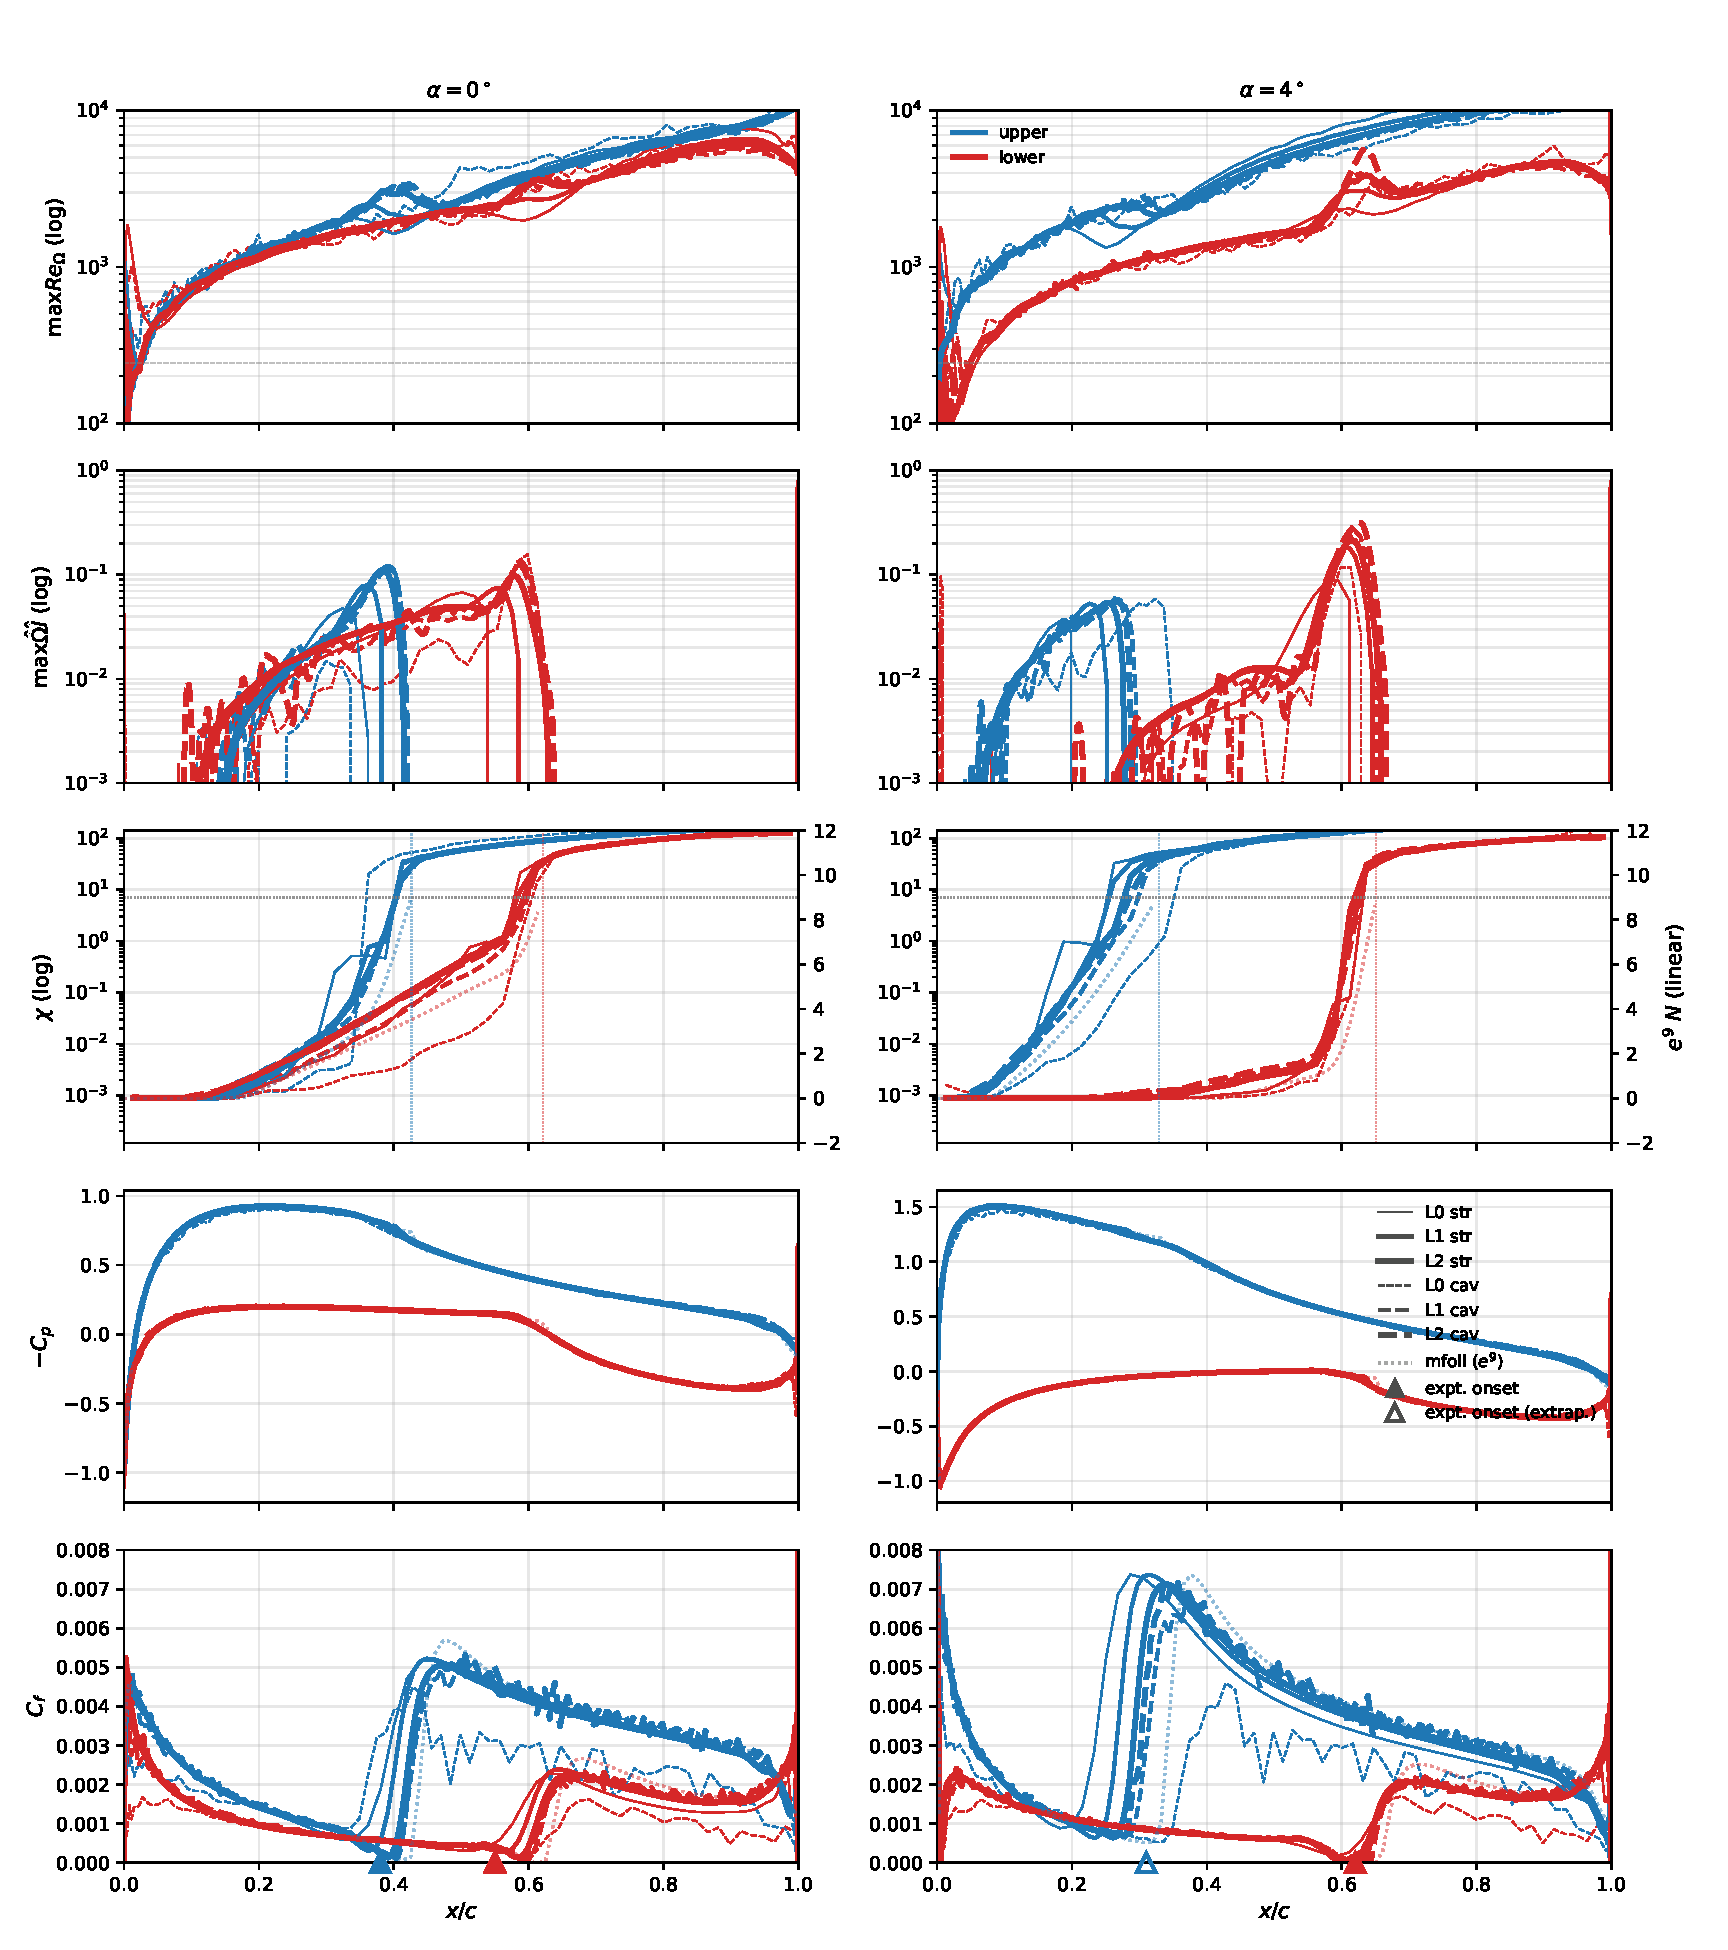
\includegraphics[width=0.95\textwidth]{nlf_cf_lowalpha.pdf}
  \caption{NLF(1)-0416 surface distributions at $\alpha\!\in\!\{0^\circ,4^\circ\}$,
  $Re\!=\!4\!\times\!10^6$, $\chi_\infty\!=\!8.76\!\times\!10^{-4}$. \emph{Top row:}
  in-BL maximum modified-viscosity ratio $\chi\!=\!\max_y\tilde\nu/\nu$ on a log
  axis (left), with mfoil's amplification factor $N$ on a linear axis (right);
  the two axes are linked by $N\!=\!\ln(\chi/\chi_\infty)$, so a unit on the
  right matches one $e$-fold on the left. Vertical dotted lines mark mfoil's
  transition $x_\mathrm{tr}$ on each surface. \emph{Middle row:} $-C_p$;
  \emph{bottom row:} $|C_f|$. Color encodes the surface (upper blue, lower red);
  line style encodes the mesh family (structured O-grid: solid, unstructured
  cavity: dashed); line thickness encodes the refinement level (L0 thinnest,
  L2 thickest). Dotted curves are the mfoil $e^9$ reference. Surfaces are
  separated by walking the airfoil contour via mesh connectivity and splitting
  at the geometric LE/TE extrema; this is essential on the NLF because the
  reflex camber places the lower surface above the chord line over the aft
  region, so a sign-of-$z$ partition interleaves the two surfaces. At
  $\alpha\!=\!0^\circ$ both surfaces transition near $x/c\!\approx\!0.45$,
  recovering the low-drag bucket; at $\alpha\!=\!4^\circ$ the upper-surface
  transition has marched forward to $x/c\!\approx\!0.30$ while the lower stays
  near design. The amplification curves (top) and the transition locations on
  $C_f$ track the $e^9$ envelope to within $\sim\!0.03$--$0.05$ chord on both
  surfaces, both meshes, and at every refinement level from L0 ($N{\approx}200$
  surface points) to L2 ($N{=}800$).}
  \label{fig:nlfcflow}
\end{figure}

\begin{figure}[tp]
  \centering
  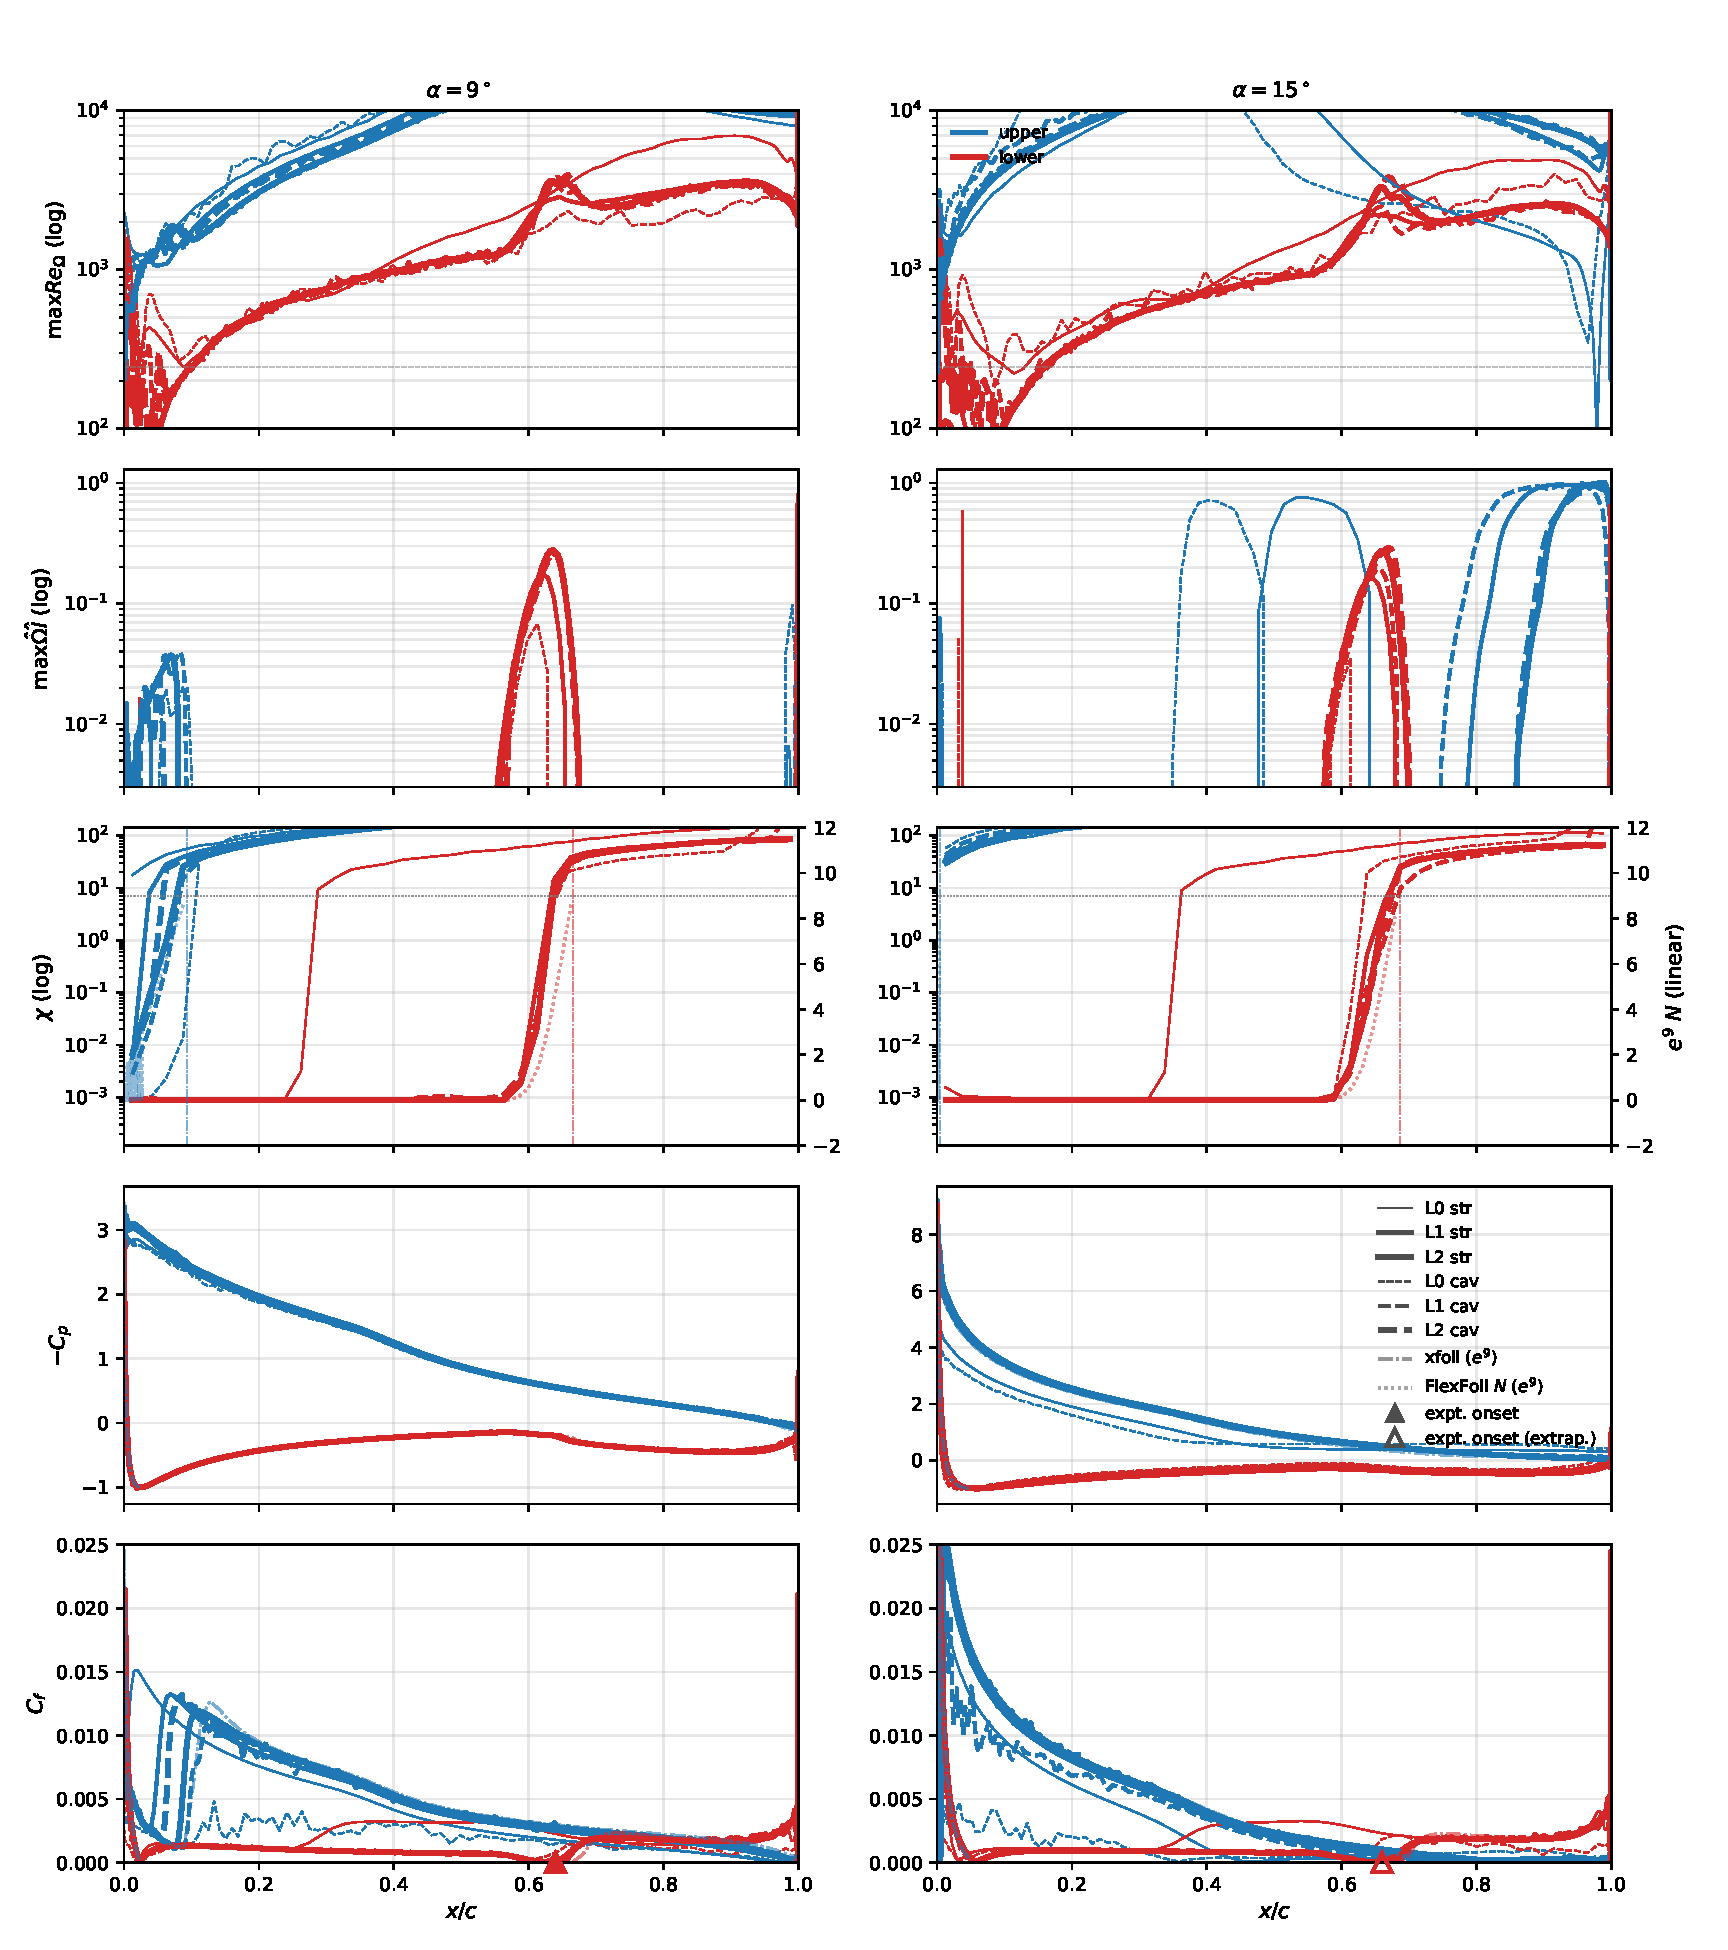
\includegraphics[width=0.95\textwidth]{nlf_cf_highalpha.pdf}
  \caption{As Fig.~\ref{fig:nlfcflow}, at $\alpha\!\in\!\{9^\circ,15^\circ\}$.
  The upper-surface transition has marched to $x/c\!\lesssim\!0.05$ at
  $\alpha\!=\!9^\circ$ and is at the LE by $\alpha\!=\!15^\circ$, while the
  lower transition remains aft of mid-chord. The L0 unstructured under-resolves
  the LE suction peak by $\sim\!1$ in $-C_p$ at $\alpha\!=\!15^\circ$ (thin
  dashed blue); L1/L2 collapse on both grids. The high-incidence cases are an
  unforgiving test of the amplification model under a strong adverse gradient:
  $\chi$ rises through $c_{v1}$ within the first few percent of chord on the
  upper surface, but the model still resolves a finite laminar dip and the
  laminar/turbulent handover stays at one chordwise location across the
  refinement series.}
  \label{fig:nlfcfhigh}
\end{figure}

The skin friction (Figs.~\ref{fig:nlfcflow}--\ref{fig:nlfcfhigh}, bottom rows)
follows the laminar branch upstream of the transition front and recovers a
turbulent level downstream, on both surfaces and at every operating point. The
chordwise location of the rise tracks the $e^9$ reference to within $\sim\!5\%$
of chord across the range $0\!\le\!\alpha\!\le\!15^\circ$; both surfaces and
both mesh families agree at L1 and L2. The pressure distributions (middle rows)
are essentially identical between L1 and L2 on each grid, including the strong
leading-edge suction at $\alpha\!=\!15^\circ$ where $-C_{p,\max}\!\approx\!8$:
the only visible refinement effect is L0 unstructured under-predicting the LE
peak by $\sim\!1$ in $-C_p$ at $\alpha\!=\!15^\circ$ (a leading-edge
$y^+$/resolution effect that the L1 mesh removes).

\begin{figure}[tp]
  \centering
  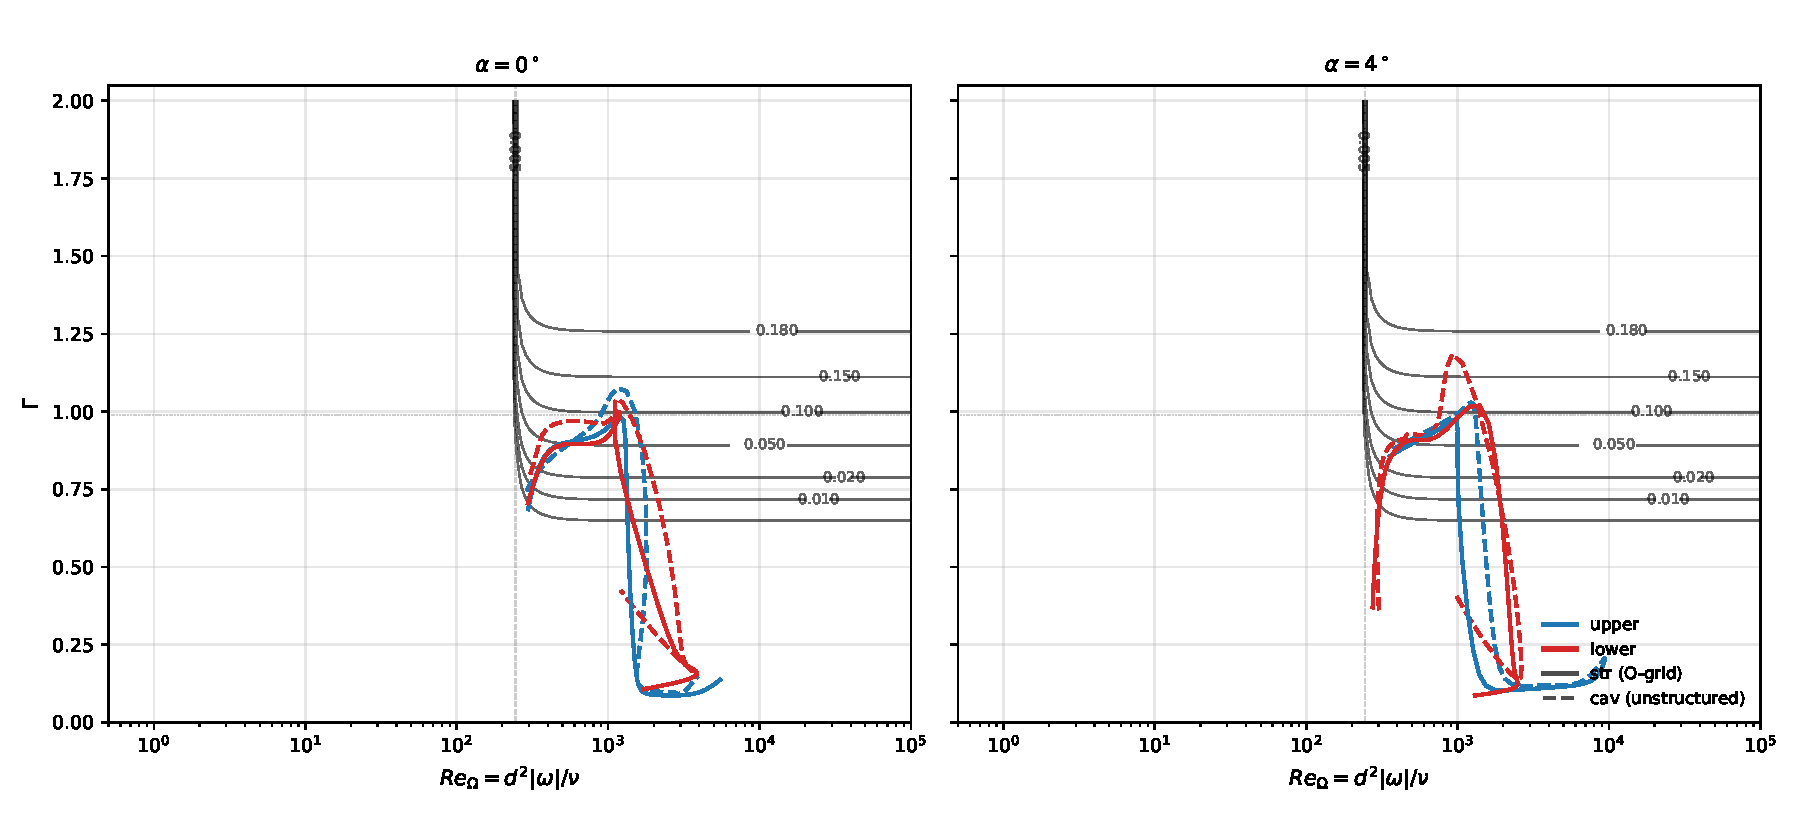
\includegraphics[width=0.49\textwidth]{nlf_landscape_lowalpha.pdf}\hfill
  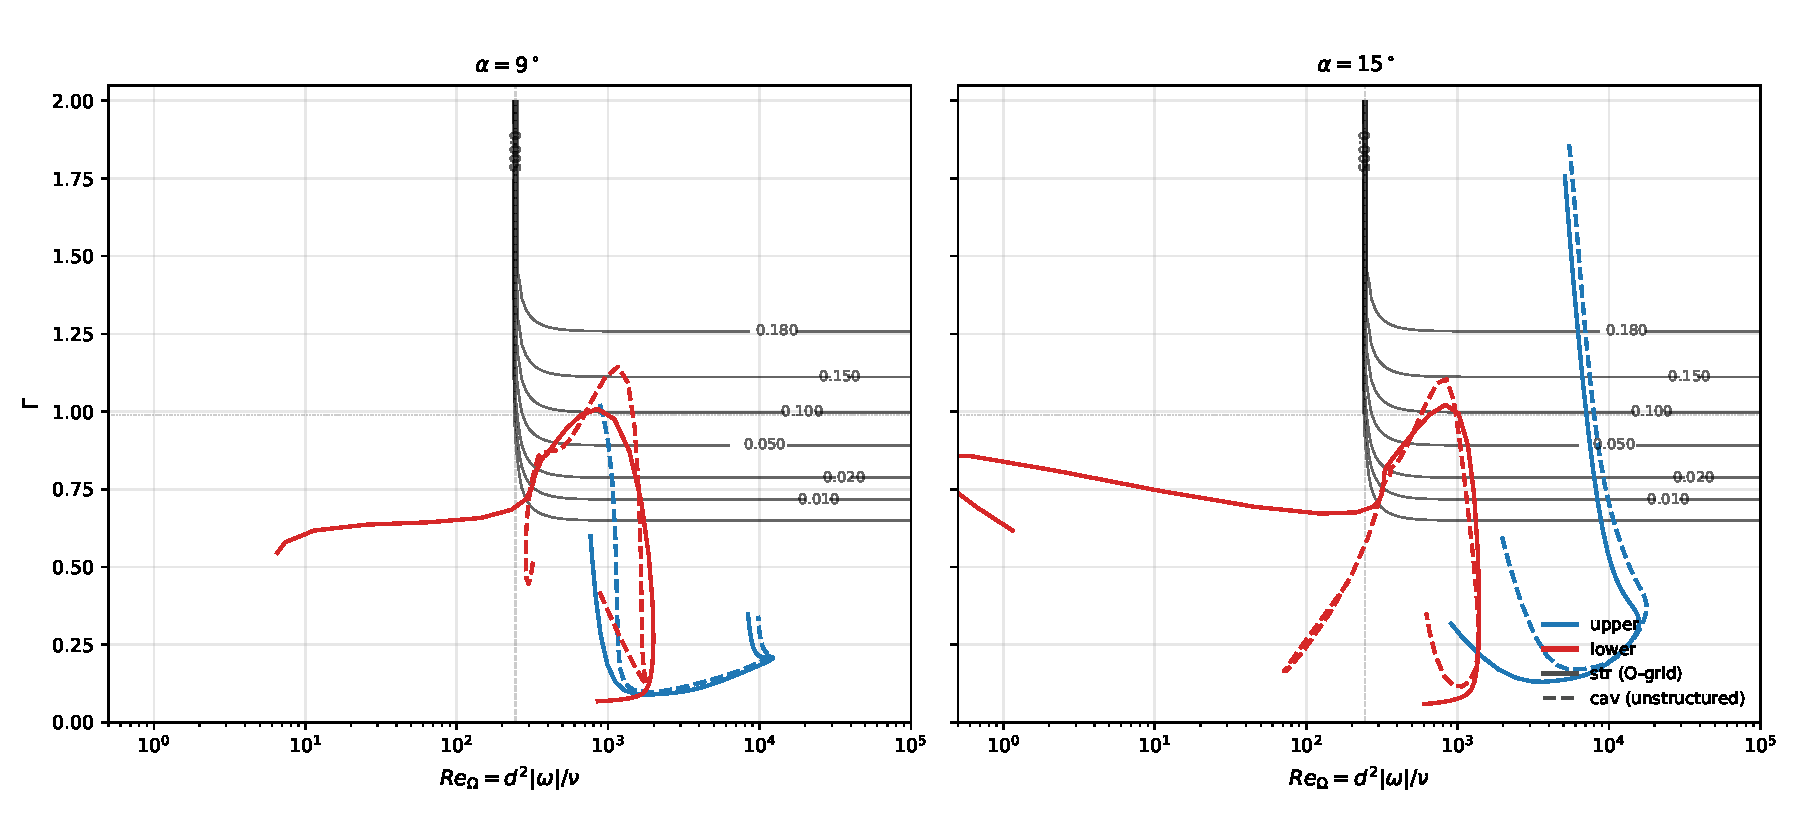
\includegraphics[width=0.49\textwidth]{nlf_landscape_highalpha.pdf}
  \caption{Amplification-rate landscape $a(Re_\Omega,\Gamma)$ and the path each
  NLF(1)-0416 boundary layer traces through it, at L1 resolution. Black contours
  are $a$; the dashed red vertical line is the cliff floor
  $Re_\Omega^{\mathrm{f}}\!=\!100$ ($\Gamma$-independent). The dotted
  horizontal line is the sigmoid center $g_c\!=\!1.572$. Each colored curve is the locus of $(Re_\Omega,\Gamma)$
  at the wall-normal location of peak kernel $a\omega$ as $x/c$ varies, with
  upper surface in blue and lower in red. Both mesh families collapse onto the
  same trajectory at every $\alpha$, including the high-incidence cases on the
  right where the upper-surface boundary layer accelerates rapidly through the
  high-rate corridor and ignites by $x/c\!\approx\!0.02$.}
  \label{fig:nlflandscape}
\end{figure}

\begin{figure}[tp]
  \centering
  
\includegraphics[width=0.49\textwidth]{nlf_convergence_lowalpha.pdf}\hfill
  
\includegraphics[width=0.49\textwidth]{nlf_convergence_highalpha.pdf}
  \caption{Residual and force-coefficient histories for the twenty-four
  NLF(1)-0416 cases ($\alpha\!\in\!\{0^\circ,4^\circ,9^\circ,15^\circ\}$ $\times$
  three refinement levels $\times$ two mesh families). Top row: continuity
  (solid) and $\tilde\nu$ (dashed) residuals; bottom row: $C_L$ and $C_D$
  histories. Line thickness encodes the refinement level (L0 thin, L2 thick);
  line style encodes the mesh family. All twenty-four cases reach a steady
  state with both residuals descending several orders of magnitude; the
  high-incidence cases ($\alpha\!=\!9^\circ,15^\circ$) require proportionally
  more pseudo-time steps but exhibit no stagnation or limit-cycle behavior.
  The convergence behavior here is achieved with the $\max$-blend production
  of Eq.~\eqref{eq:blend} (see Sec.~\ref{sec:blendnlf}) and with the
  laminar-slowdown factor $f_\mathrm{slow}\!=\!0.01$ that damps the
  natural-transition feedback discussed below.}
  \label{fig:nlfconv}
\end{figure}

The amplification-rate landscape (Fig.~\ref{fig:nlflandscape}) collapses the
twenty-four cases onto a single physical picture: both surfaces enter the
landscape from the low-$Re_\Omega$, low-$\Gamma$ corner near the LE,
follow the favorable-gradient rooftop along $\Gamma\!<\!g_c$ with the
amplification rate kept small, and ignite where the trajectory crosses
$\Gamma\!=\!g_c$ near the start of pressure recovery. The two mesh families
trace the same curve in $(Re_\Omega,\Gamma)$ space at every $\alpha$. At
$\alpha\!=\!15^\circ$ the upper-surface curve traverses the corridor within
the first few percent of chord, igniting almost immediately at the LE, while
the lower-surface curve lingers in the low-rate corner past mid-chord.

\subsection{Marginal natural transition and the production blend}\label{sec:blendnlf}

The NLF(1)-0416 exposes a coupling that fixes the form of the production blend
\eqref{eq:blend}. Its long favorable-gradient rooftop keeps the boundary layer near
neutral over an extended chord fraction, so the amplification ignites only where
recovery begins ($\Gamma\!\to\!1$) and the transition location is marginal. On the
fine structured O-grid, a \emph{convex} blend $\sigma_t P_\mathrm{SA}+(1-\sigma_t)
P_\mathrm{AFT}$ then fails to reach a steady state: the transition front breathes with
a $\pm$few-percent drag oscillation at fixed pseudo-time settings. The oscillation is
not numerical---it is invariant to the pseudo-time step---but a genuine feedback. Its
signature is \emph{global}: the surface pressure at the leading edge, far upstream of
transition, oscillates in near-perfect anti-phase with the lift coefficient
($\mathrm{corr}\approx-1$), which a local disturbance could not produce. The loop is
transition $\to$ boundary-layer displacement $\to$ Kutta circulation $\to$ effective
incidence $\to$ the pressure-gradient (shape-factor) sensitivity of the amplification
at the front $\to$ transition. Because the amplification rate depends on $\Gamma$
through a steep activation \eqref{eq:rate}, even the $\mathcal{O}(1\%)$ circulation
breathing is enough to move a marginal front; on coarser or more dissipative meshes
the feedback is damped and the issue does not appear.

The carrier of this receptivity is exactly the term the convex blend retains past
transition: the $(1-\sigma_t)P_\mathrm{AFT}$ bleed for $\chi>1$, which keeps the
\emph{pressure-sensitive} amplification weighted into the early-turbulent region where
the front lives. The $\max$ blend \eqref{eq:blend} removes it---once $\sigma_t
P_\mathrm{SA}$ overtakes amplification just past $\chi=1$, the production is purely the
pressure-\emph{insensitive} SA term---so the front carries no receptivity to the global
pressure field and the computation converges to steady state. With \eqref{eq:blend} the
O-grid NLF(1)-0416 reaches a steady solution at every incidence
(Fig.~\ref{fig:nlfconv}), the transition location agrees with the unstructured mesh
and tracks the $e^N$ reference across the polar (Fig.~\ref{fig:xtr}), and the
laminar/amplification calibration is untouched ($\max$ and convex are identical
for $\chi\le1$).

A second, weaker form of the same coupling persists with the $\max$ blend on
the unstructured cavity grid: a slow chi-front breathing whose amplitude
remains finite at long pseudo-times. A small laminar slowdown factor
$f_\mathrm{slow}\!=\!0.01$ multiplying the amplification production
geometrically through a blend variable
$\mathrm{scale}\!=\!f_\mathrm{slow}^{\,1-g_\mathrm{slow}}$ damps this residual
feedback without shifting the converged transition location. The slowdown
gate $g_\mathrm{slow}(\chi)\!=\!1\!-\!\exp\!\big(-(\chi-\chi_\mathrm{slow})/w_\mathrm{slow}\big)$
holds the slowdown FULLY ON throughout $\chi\!\in\![0,\chi_\mathrm{slow}]$
and only relaxes once $\chi$ crosses the eddy-viscosity half-saturation point;
we set $\chi_\mathrm{slow}\!=\!c_{v1}\!=\!7.1$ (the slowdown gate spans the
entire breathing $\chi\!\in\![1,c_{v1}]$ band where the transition-front
receptivity actually lives) with $w_\mathrm{slow}\!=\!4$. With both
modifications --- the $\max$ production blend and the $c_{v1}$-anchored
geometric slowdown --- all twenty-four cases of Fig.~\ref{fig:nlfconv}
converge to a steady state with no residual limit cycle.

\section{Airfoil Validation: NACA~0012}\label{sec:airfoil}

The model is applied to a NACA~0012 at $Re=10^6$, $M=0.2$, $\alpha=0^\circ$, on the
quasi-two-dimensional unstructured mesh of Fig.~\ref{fig:mesh}, generated by an
in-house Delaunay mesher driven by an a-priori Spalding
boundary-layer metric ($1.1\!\times\!10^5$ nodes, $400$ points around the
airfoil, near-wall spacing targeting $y^+\!\approx\!0.25$, growth ratio
$1.1$, farfield radius $100\,c$). To admit
a laminar boundary layer the freestream ratio is set low,

\begin{figure}[tp]
  \centering
  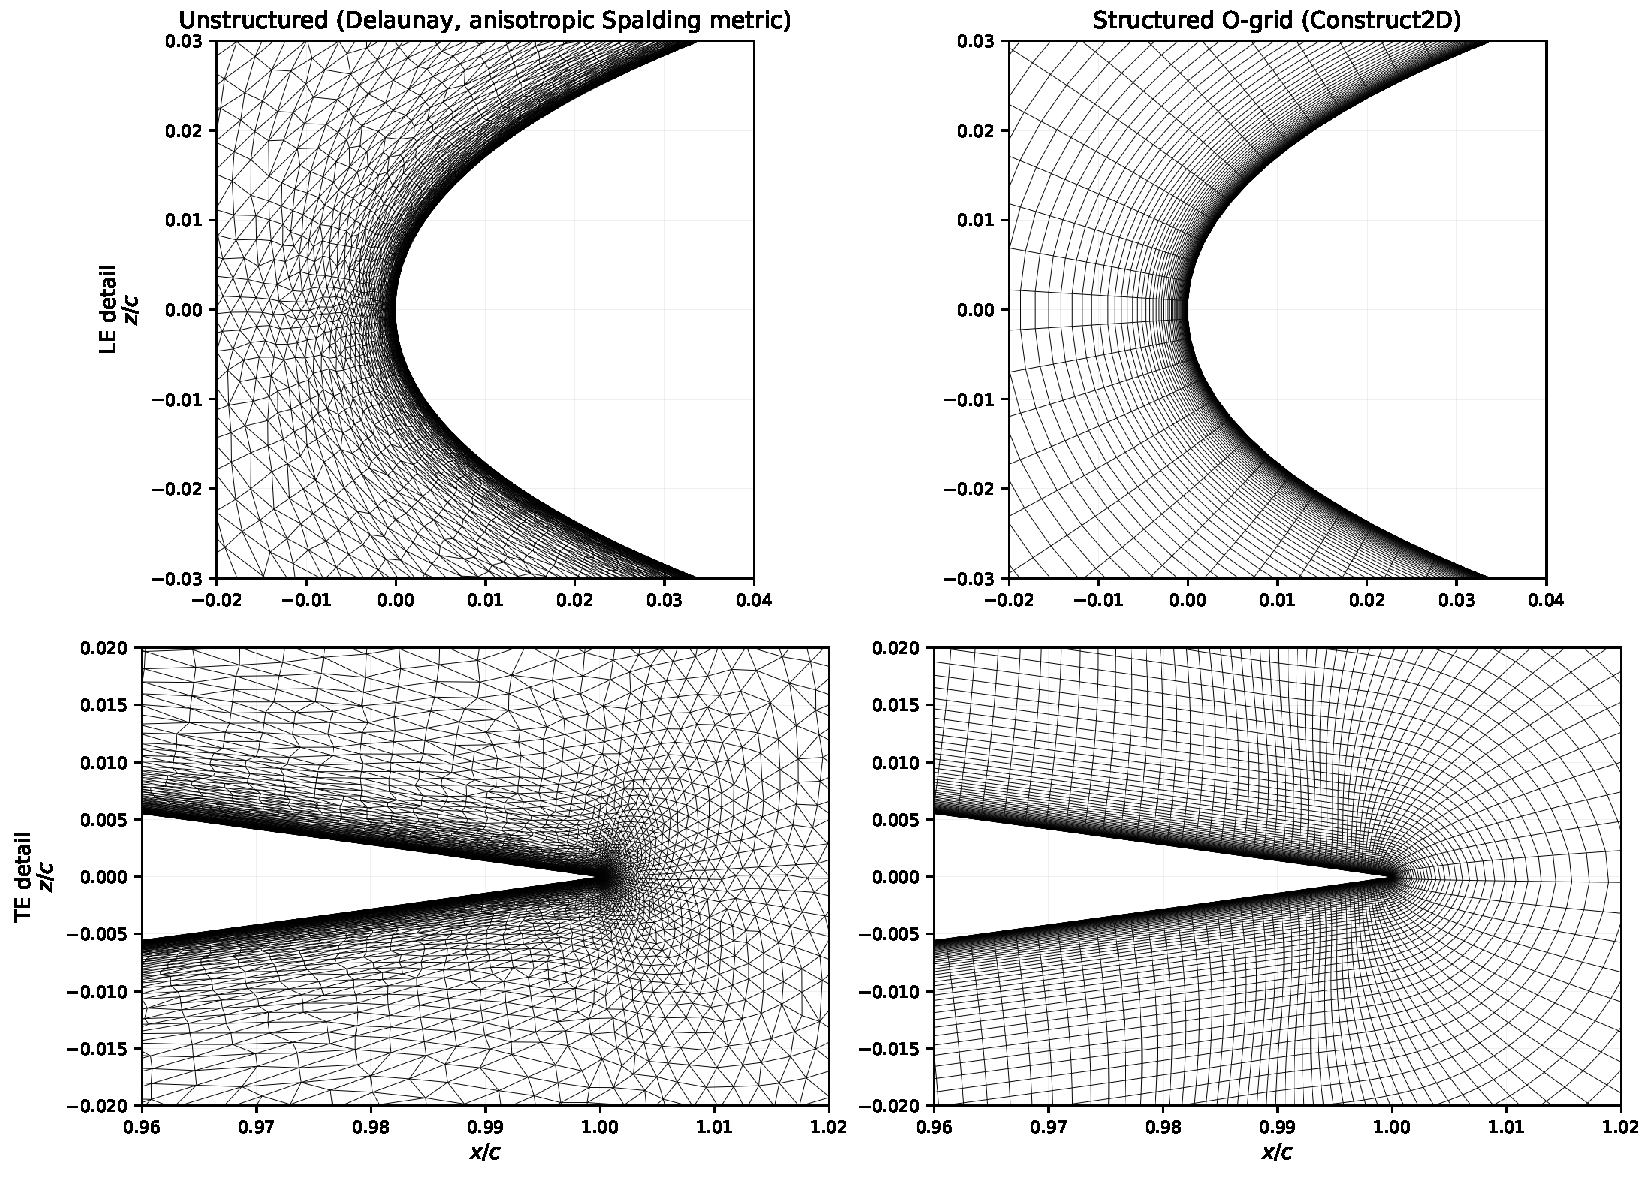
\includegraphics[width=0.95\textwidth]{mesh.pdf}
  \caption{The two NACA~0012 meshes used in this study (in-plane slice; L1
  refinement level). \emph{Top row: leading-edge detail; bottom row: trailing-edge
  detail.} \emph{Left column:} the unstructured anisotropic mesh (Delaunay with
  Spalding-style near-wall metric), included as an \emph{adversarial} test for the
  present model. The mesher attempts to align triangular prism layers with the
  wall but many near-wall triangles are nearly degenerate,
  with interior angles approaching $0^\circ/0^\circ/180^\circ$---sliver elements
  in which the gradient stencil is severely skewed; these layers are also the
  source of the tangential $C_f$ staggering observed below. The TE detail
  shows the result after pinning the chord-direction contour spacing at
  $h_\mathrm{TE}\!=\!h_0$ and modifying the mesher's tangential metric to use
  the LOCAL contour-segment length rather than a single global constant
  ($h_\mathrm{wall}$); without these fixes the unstructured TE region produces
  a fan of sliver elements spanning $h_\mathrm{wall}\!\sim\!10^3 h_0$
  tangentially and a non-monotonic $C_L$ at L1 (Sec.~\ref{sec:gridconv}).
  \emph{Right column:} the structured O-grid (Construct2D), with fully
  wall-aligned quad-prism cells and staggering-free. Both resolve the
  boundary layer to $y^+\!\lesssim\!0.4$ at the leading edge; the results below are computed
  on both, and the unstructured mesh is reported as a worst-case stress test
  of how the transition model behaves on a strongly anisotropic, partly
  degenerate near-wall stencil.}
  \label{fig:mesh}
\end{figure}
$\chi_\infty=0.02$;
this is compared against standard SA at the fully turbulent $\chi_\infty=3$ and, as a
control, standard SA at the \emph{same} $\chi_\infty=0.02$. Table~\ref{tab:drag}
reports the converged force coefficients and Fig.~\ref{fig:cf} the chordwise
skin-friction distribution.

\begin{table}[t]
  \centering
  \caption{NACA~0012 drag breakdown ($Re=10^6$, $M=0.2$, $\alpha=0^\circ$), on
  the L1-refinement structured O-grid ($1.3\!\times\!10^5$ nodes) and the L1
  unstructured mesh ($1.1\!\times\!10^5$ nodes). The two grids agree on the
  SA-AF drag to within $0.5\%$.}
  \label{tab:drag}
  \begin{tabular}{llccc}
    \toprule
    Model & Grid & $C_D$ & $C_{D,\mathrm{pressure}}$ & $C_{D,\mathrm{friction}}$ \\
    \midrule
    SA (turbulent), $\chi_\infty{=}3$    & O-grid & 0.01084 & 0.00204 & 0.00880 \\
    SA-AF, $\chi_\infty{=}0.02$          & O-grid & \textbf{0.00746} & 0.00140 & \textbf{0.00605} \\
    \addlinespace[2pt]
    SA (turbulent), $\chi_\infty{=}3$    & unstructured & 0.01095 & 0.00215 & 0.00879 \\
    SA-AF, $\chi_\infty{=}0.02$          & unstructured & \textbf{0.00742} & 0.00149 & \textbf{0.00593} \\
    \bottomrule
  \end{tabular}
\end{table}

Standard SA is insensitive to the freestream level---it bypasses to
turbulence from the leading edge, giving the same fully turbulent drag at
$\chi_\infty=0.02$ as at $\chi_\infty=3$ to within $1\%$---so only the turbulent
$\chi_\infty=3$ result is reported, and the reduction below is due to the transition
model, not to the lowered freestream. SA-AF instead sustains a laminar run: the skin
friction (Fig.~\ref{fig:cf}, bottom-left) follows the laminar trend to a minimum
near $x/c\approx0.5$ and then rises to the turbulent level, a signature the
turbulent computation (dash-dot) does not show. Friction drag falls by $31\%$ and
total drag by $31\%$ relative to turbulent SA at the same condition on the O-grid,
and the corresponding reductions on the unstructured mesh are $33\%$ and $32\%$;
the two grids agree on the SA-AF total drag to within $0.5\%$. The small-amplitude
($\sim$few percent) oscillations in the unstructured $C_f$ are a tangential
staggering of the node-centered scheme on the triangulated near-wall layers
(Fig.~\ref{fig:mesh}); they are insensitive to $y^+$, leave the friction
integral unchanged within $0.1\%$, and vanish on the O-grid. This is the
zero-incidence, maximum-laminar-fraction case; the laminar run shortens with
lift.

The case converges to steady state without special treatment.
Figure~\ref{fig:conv} shows the residual histories of SA-AF across the L0--L2
grid-refinement series on both mesh families. Both the continuity and the
$\tilde\nu$ residuals drop several orders of magnitude in $\sim\!2\!\times\!10^4$
pseudo-time steps, with the transient hump near step $10^4$ corresponding to the
laminar-to-turbulent handover of the model and reproducing on both grids. No
stagnation or stability penalty is observed at any refinement level---the
practical payoff of the analytic Jacobian of Sec.~\ref{sec:model}.

\subsection{Grid convergence}\label{sec:gridconv}
Every airfoil result is computed on two unrelated mesh families---an anisotropic
unstructured mesh and a structured O-grid (Construct2D)---and
Figs.~\ref{fig:cf}, \ref{fig:conv}, \ref{fig:polar}, and~\ref{fig:xtr}
overlay both. The unstructured family is deliberately retained as an \emph{adversarial}
discretization, with the sliver near-wall triangles of Fig.~\ref{fig:mesh} that the
prism extruder cannot eliminate; the O-grid is the controlled, fully wall-aligned
reference. Both families are built to a leading-edge $y^+\!\lesssim\!0.4$, which is
not free: the unstructured mesher derives its first-cell height from a turbulent flat-plate
friction estimate, which under-predicts the laminar leading-edge wall shear by a
factor of $\sim\!2$--$3$ and overshoots $y^+$ at the LE by that ratio; an explicit
first-cell override pulls the LE $y^+$ back into target range and the unstructured LE skin
friction then agrees with the integral-method reference and with the O-grid. Once the
LE is resolved on both, the pressure distributions, the polar lift and pressure
drag, the laminar skin-friction profile inboard of transition, and the transition-vs.\
incidence trend all agree closely between the two grids, and the structured grid is
additionally free of the tangential $C_f$ staggering of Fig.~\ref{fig:mesh}.

A systematic refinement study (Fig.~\ref{fig:gridconv}) uses three unstructured meshes
(L0--L2, $3.1\times10^4$ to $3.9\times10^5$ nodes) and three O-grid meshes
(L0--L2, $3.2\times10^4$ to $5.1\times10^5$ nodes) at $\alpha=4^\circ$, where the
favorable-to-adverse pressure gradient pins the transition robustly. The series
refines every discretization length scale by a factor of two per level: surface
point count, first-cell height $h_0$, growth-ratio offset $(g-1)$, the TE contour
spacing $h_\mathrm{TE}\!=\!h_0$ (so the corner cells stay isotropic), and the
TE-to-bulk geometric ramp ratio $r_\mathrm{TE}$ from $2.0$ at L0 to
$1.25$ at L2 (so the local cell size at fixed chord-distance from the TE also
halves). This is a proper isotropic refinement in every direction at every
location---not the more common practice of refining only the wall-normal
direction or only the first cell.

A complication particular to the unstructured mesher must be addressed: its a-priori
Spalding-style metric prescribes the wall-tangential cell size from a single
global constant ($h_\mathrm{wall}$, conventionally also the BL extent),
independent of the user-supplied contour discretization. With that constant the
mesher ignores small $h_\mathrm{TE}$ in the contour and inserts cells of size
$h_\mathrm{wall}$ tangentially at the wall regardless. We modified the metric
locally to use the LOCAL contour-segment length as the tangential cell size at
the wall (see TE detail in Fig.~\ref{fig:mesh}); this preserves the user's
intended TE discretization in the actual mesh.

With these changes (TE-proper contour and segment-length-respecting metric), the
adversarial unstructured series converges monotonically and tightly:
$C_L$ marches $0.4231\!\to\!0.4264\!\to\!0.4277$,
$C_D$ marches $0.00855\!\to\!0.00874\!\to\!0.00869$,
$C_{D,p}$ marches $0.00321\!\to\!0.00274\!\to\!0.00252$ (matching O-grid
$C_{D,p}=0.00249$ to $1\%$), and $C_{M,y}$ marches
$-0.1001\!\to\!-0.1010\!\to\!-0.1014$. Even the coarsest L0
($3\!\times\!10^4$ nodes) is within $1\%$ of the L2 converged $C_L$, in stark
contrast to the original (no $h_\mathrm{TE}$ control) unstructured where L0 was $10\%$
low and L1 spiked above the trend. At L2 the adversarial unstructured and the
wall-aligned O-grid agree to $0.8\%$ in $C_L$ ($0.4277$ vs $0.4312$), $5.5\%$ in
$C_D$ ($0.00869$ vs $0.00824$), and within the transition-band width on the
upper-surface midpoint. The model thus converges consistently across two very
different near-wall stencils when both the contour discretization \emph{and} the
mesher's tangential metric respect the same local length scale.

The residual $C_D$ offset between unstructured-L2 and O-grid-L2 ($\sim\!6\%$) is a
boundary-layer gradient-stencil effect on the anisotropic triangular prism layers,
distinct from the TE issue and not fixed by $h_\mathrm{TE}$ refinement: the
gradient reconstruction across high-AR triangles renders the unstructured's $\delta_{99}$
slightly thicker than the O-grid's at matched $x_w$, leaving the amplification
integral $\int a(Re_\Omega,\Gamma)\,\omega\,dz$ a few percent shorter and the
post-transition $C_f$ a few percent higher. This is a known property of unstructured
triangle-prism BL meshing and not specific to the present transition model. The
refinement is reported at a lifting incidence by necessity: at the symmetric
$\alpha=0^\circ$ the near-zero pressure gradient pins the transition too weakly to
grid-converge on either family---a sensitivity of the natural-transition problem
itself rather than of the model.

Reaching this behavior requires one methodological choice: the interior $\tilde\nu$
field must be \emph{initialized at the laminar freestream level} $\chi_\infty$, not at
the solver's near-turbulent default. Because the SA dynamics do not relaminarize, an
elevated initial field persists from the leading edge on a fine grid---turning the
result fully turbulent independent of the amplification model---whereas a laminar start
lets the AFT term set the transition location. The $\Gamma$-dependent cliff
\eqref{eq:cliff} reinforces this by removing the residual near-wall amplification that
the bare activation (which leaves $\Gamma\!\approx\!1$ active at the wall) would
otherwise accumulate; without it the symmetric $\alpha=0^\circ$ case under-trips on the
structured grid even at production resolution.

\begin{figure}[tp]
  \centering
  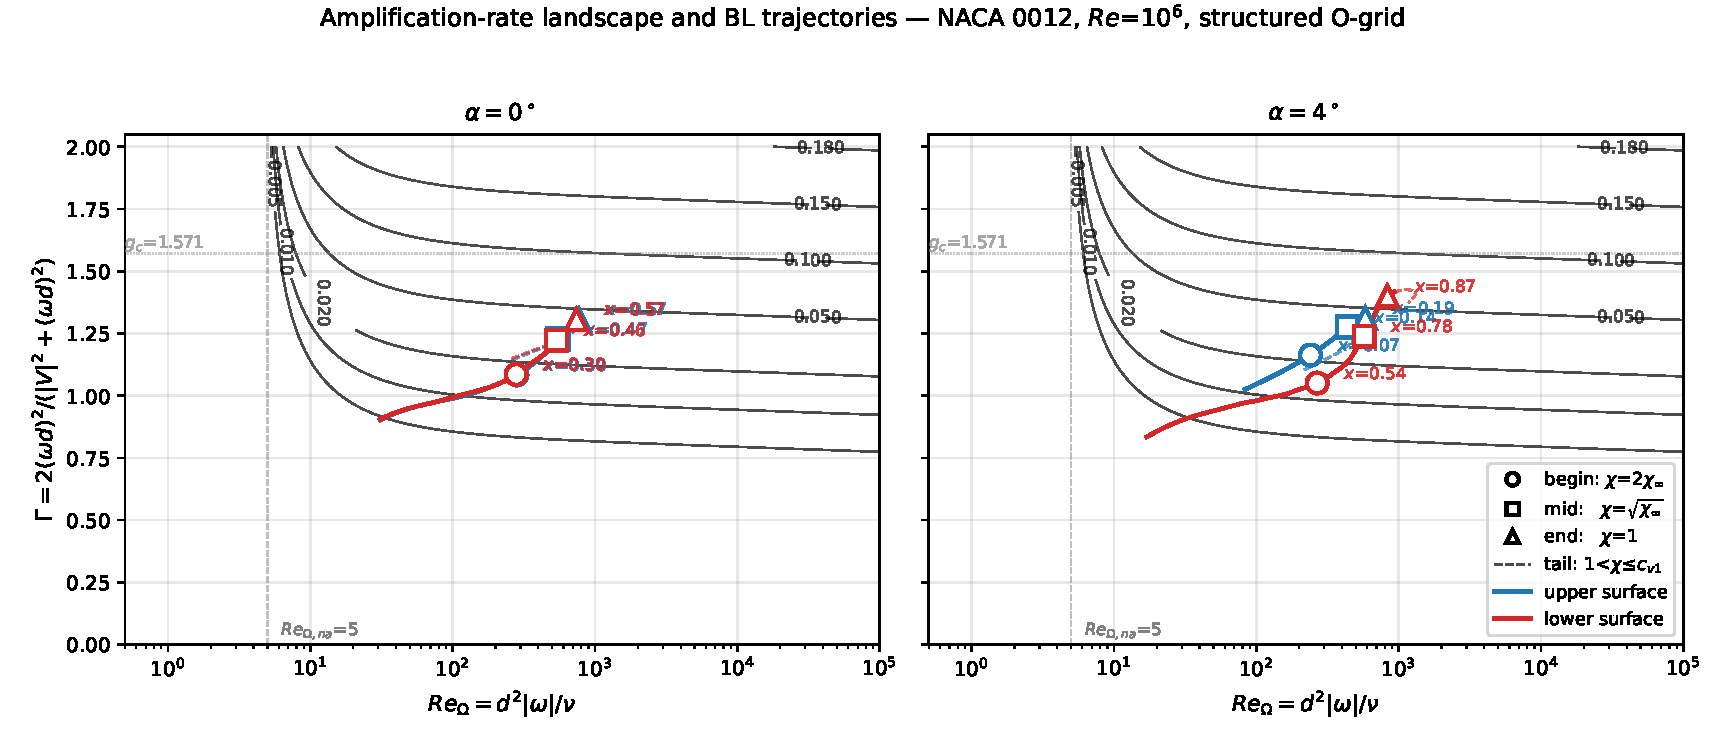
\includegraphics[width=0.95\textwidth]{landscape_trajectories.pdf}
  \caption{Amplification-rate landscape and the path each boundary layer traces
  through it. Black contours: $a(Re_\Omega,\Gamma)$ from Eq.~\eqref{eq:rate}
  with the recalibrated unified constants of Table~\ref{tab:const}; the dashed
  red curve is the $\Gamma$-dependent cliff $Re_\Omega^{\mathrm{c}}(\Gamma)$
  of Eq.~\eqref{eq:cliff} and the
  dotted horizontal line is the sigmoid center $g_c\!=\!1.572$. For each
  streamwise station we pick the wall-normal location at which the local
  kernel $a\omega$ peaks and record its $(Re_\Omega,\Gamma)$; following $x$
  along the chord traces the colored curves (upper surface in blue, lower in
  red). Markers along each curve mark, in order, the streamwise stations at
  which $\chi$ crosses $2\chi_\infty$ (beginning of the rise, $\bigcirc$),
  $\sqrt{\chi_\infty}$ (geometric mid-point of the linear-amplification
  interval $[\chi_\infty,1]$, $\square$), and $\chi\!=\!1$ ($\triangle$), the
  end of clean linear amplification: past this point the eddy-viscosity
  feedback begins to squash the boundary-layer profile toward a turbulent
  shape and the $(Re_\Omega,\Gamma)$ trajectory loops around (drawn as a thin
  dashed tail extending to $\chi\!=\!c_{v1}\!=\!7.1$, where $f_{v1}\!=\!\tfrac12$).
  At $\alpha\!=\!0^\circ$ (left) the two surfaces overlap by symmetry; at
  $\alpha\!=\!4^\circ$ (right) the upper-surface trajectory accelerates
  through the rise by $x/c\!\approx\!0.19$ while the lower lingers in the
  low-$Re_\Omega$ low-rate corner until $x/c\!\approx\!0.5$, reaching
  $\chi\!=\!1$ only near $x/c\!\approx\!0.87$.}
  \label{fig:landscape}
\end{figure}

\begin{figure}[tp]
  \centering
  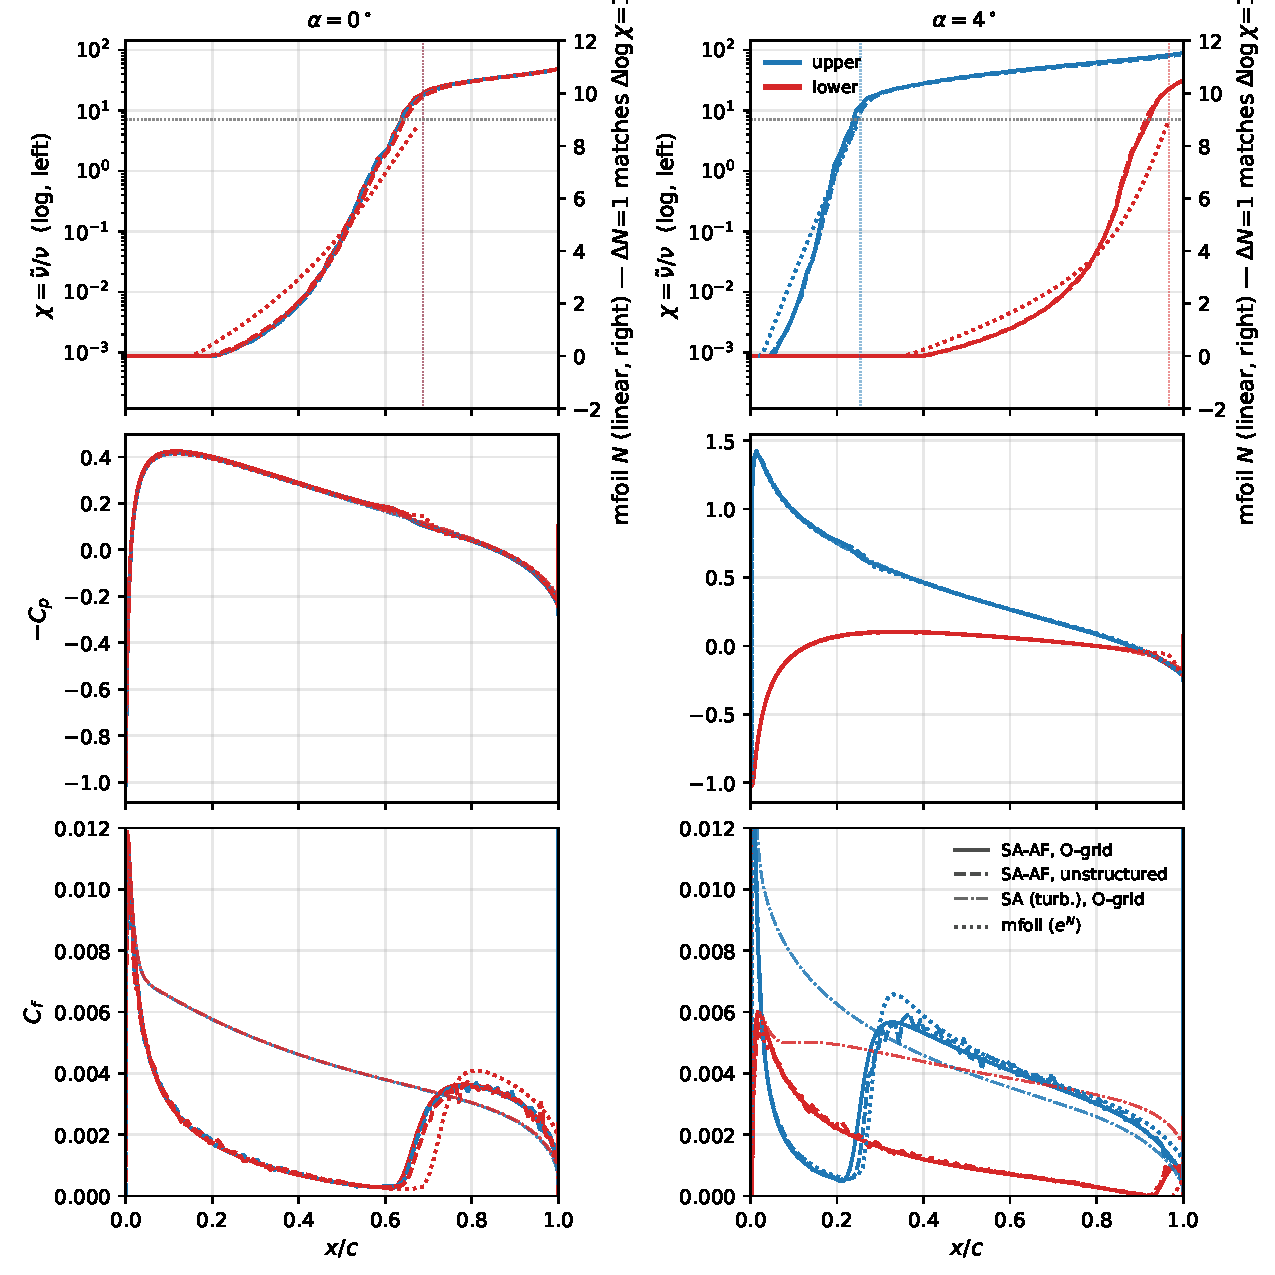
\includegraphics[width=0.95\textwidth]{naca0012_cf.pdf}
  \caption{NACA~0012 at $\alpha=0^\circ$ (left column) and
  $\alpha=4^\circ$ (right column), on a $1.1\!\times\!10^5$-node unstructured
  mesh and a $1.3\!\times\!10^5$-node structured O-grid,
  $\chi_\infty\!=\!c_{v1}\,e^{-9}\!\approx\!8.76\!\times\!10^{-4}$. The freestream is
  anchored to the rigorous half-saturation criterion: at $\chi\!=\!c_{v1}\!=\!7.1$ the
  SA eddy-viscosity function $f_{v1}(\chi)\!=\!\chi^3/(\chi^3+c_{v1}^3)$ is exactly
  $\tfrac12$, so $\chi_\infty\!=\!c_{v1}\,e^{-N_\mathrm{crit}}$ makes
  $N_\mathrm{crit}\!=\!\ln(c_{v1}/\chi_\infty)$ the amplification at which $\tilde\nu$
  has grown by $e^9$ from its freestream seed and the eddy viscosity is half-engaged
  --- the natural correspondence to the canonical $N_\mathrm{crit}\!=\!9$ envelope.
  \emph{Top row}: in-BL maximum modified-viscosity ratio
  $\chi\!=\!\max_y\tilde\nu/\nu$ on a log scale (left axis), with mfoil's
  amplification factor $N$ on a linear scale (right axis); the two axes are
  linked exactly by $N\!=\!\ln(\chi/\chi_\infty)$, so a unit on the right
  matches one e-fold on the left. The dashed grey lines mark
  $\chi\!=\!c_{v1}$ (left) and $N\!=\!9$ (right) at the same vertical position;
  the vertical dotted lines mark mfoil's transition $x_\mathrm{tr}$. \emph{Middle row}: $-C_p$ on the upper (blue)
  and lower (red) surfaces. \emph{Bottom row}: $|C_f|$. Line style
  distinguishes the solver/grid (SA-AF O-grid: solid, SA-AF unstructured:
  dashed, SA fully turbulent: dash-dot, mfoil $e^9$: dotted). SA-AF transition
  tracks the mfoil $e^9$ envelope on both surfaces and at both incidences;
  fully turbulent SA stays turbulent from the leading edge. The structured grid
  is free of the tangential $C_f$ staggering seen on the triangulated near-wall
  layers of the unstructured mesh.  The mfoil $e^N$ reference is also at
  $N_\mathrm{crit}\!=\!9$.}
  \label{fig:cf}
\end{figure}

\begin{figure}[tp]
  \centering
  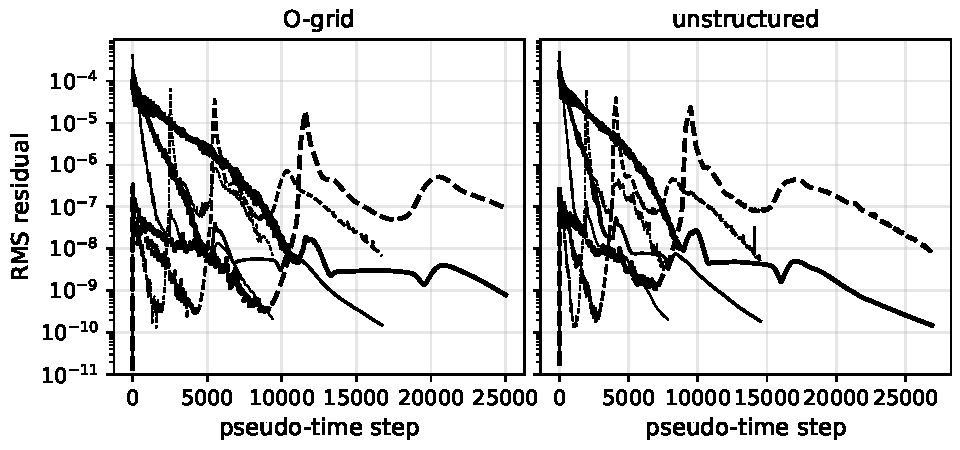
\includegraphics[width=0.95\textwidth]{convergence.pdf}
  \caption{Residual convergence of SA-AF at $\alpha=4^\circ$, $Re=10^6$,
  $\chi_\infty=0.02$ across the L0--L2 grid-refinement series, with the two mesh
  families (left: O-grid, right: unstructured) plotted in separate panels.
  Continuity residual is solid, $\tilde\nu$ residual is dashed; line thickness
  encodes the refinement level (thin = L0, medium = L1, thick = L2). Both grid
  families drive both residuals monotonically to $\sim\!10^{-9}$ at every level,
  with the finer meshes requiring proportionally more pseudo-time steps but no
  stagnation or stability penalty.}
  \label{fig:conv}
\end{figure}

\begin{figure}[tp]
  \centering
  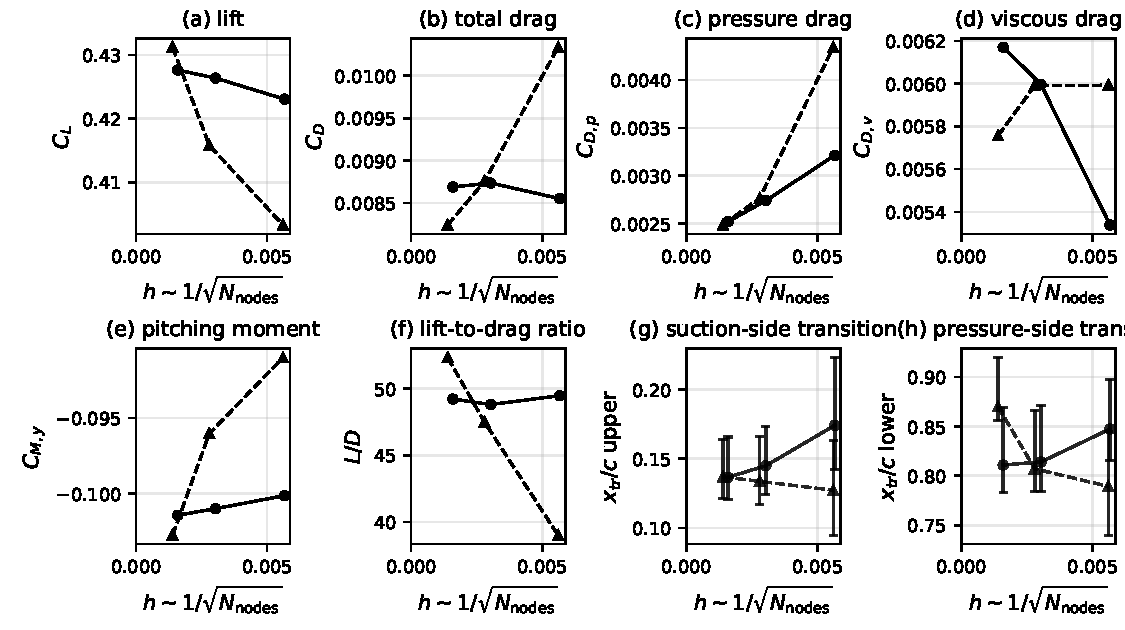
\includegraphics[width=0.95\textwidth]{proper_grid_convergence_L3.pdf}
  \caption{Grid-refinement study at $\alpha=4^\circ$, $Re=10^6$, $\chi_\infty=0.02$,
  on properly refined meshes: every discretization length scales by a factor of
  two per level (surface point count, first-cell height $h_0$, growth-ratio offset
  $(g-1)$, the chord-direction TE contour spacing $h_\mathrm{TE}\!=\!h_0$, and
  the TE-to-bulk geometric ramp ratio $r_\mathrm{TE}$). The unstructured
  series (solid line, circles, L0--L2) spans $3.1\!\times\!10^4$ to
  $3.9\!\times\!10^5$ nodes; the O-grid (dashed line, triangles, L0--L2) spans
  $3.2\!\times\!10^4$ to $5.1\!\times\!10^5$ nodes. Eight quantities are
  shown: \emph{(a)} lift coefficient, \emph{(b)} total drag, \emph{(c)} pressure
  drag, \emph{(d)} viscous (skin-friction) drag, \emph{(e)} pitching moment about
  the LE, \emph{(f)} $L/D$, \emph{(g, h)} upper- and lower-surface transition
  midpoint with error bars spanning the $10\%$--$90\%$ $C_f$-rise interval. With
  the TE-proper contour, the segment-length-respecting metric, and the
  proper-everywhere refinement, the adversarial unstructured converges tightly and
  monotonically: even the coarsest L0 is within $1\%$ of L2 in $C_L$, and at L2
  the unstructured and O-grid agree to $0.8\%$ in $C_L$ ($0.4277$ vs $0.4312$), $5.5\%$
  in $C_D$ ($0.00869$ vs $0.00824$), and within the transition-band width on the
  upper-surface midpoint.}
  \label{fig:gridconv}
\end{figure}

\subsection{Comparison with the $e^N$ method across incidence}\label{sec:sweep}

To assess the model beyond a single operating point, an angle-of-attack sweep
($\alpha=-2^\circ$ to $8^\circ$) was computed for the NACA~0012 and for the
NLF(1)-0416 natural-laminar-flow airfoil at $Re=10^6$, $M=0.2$, $\chi_\infty=0.02$,
and compared against \texttt{mfoil}---a viscous--inviscid panel method with the
$e^N$ envelope transition criterion, in the manner of XFOIL
\cite{drela_giles_1987, drela_xfoil_1989}---at the matched critical factor
$N_\mathrm{crit}\!=\!\ln(c_{v1}/\chi_\infty)\!\approx\!5.87$ (so that
$\chi_\infty\!=\!c_{v1}e^{-N_\mathrm{crit}}\!\approx\!0.02$).

Figure~\ref{fig:polar} shows the drag polars, with fully turbulent SA included as
a reference. SA-AF reproduces the lift--incidence relation of the $e^N$ reference
closely on both airfoils and recovers the characteristic low-drag bucket of the NLF
airfoil. Its drag lies between fully turbulent SA and the $e^N$ reference: the
reduction relative to turbulent SA is the laminar benefit, while the residual
offset above the $e^N$ values reflects the higher turbulent skin friction of
the RANS closure relative to an integral method. The $\alpha=4^\circ$ panel of Fig.~\ref{fig:cf} (bottom-right) isolates
the origin of this offset: the surface pressure distributions of SA-AF and the
$e^N$ reference (top-right) are nearly indistinguishable, so the lift and pressure
drag agree, but the post-transition turbulent $C_f$ from SA-AF lies above the
integral-method value. The drag offset in Fig.~\ref{fig:polar} is therefore a
turbulent-skin-friction effect of the RANS closure, not an error in the pressure
field or the transition location.

\begin{figure}[tp]
  \centering
  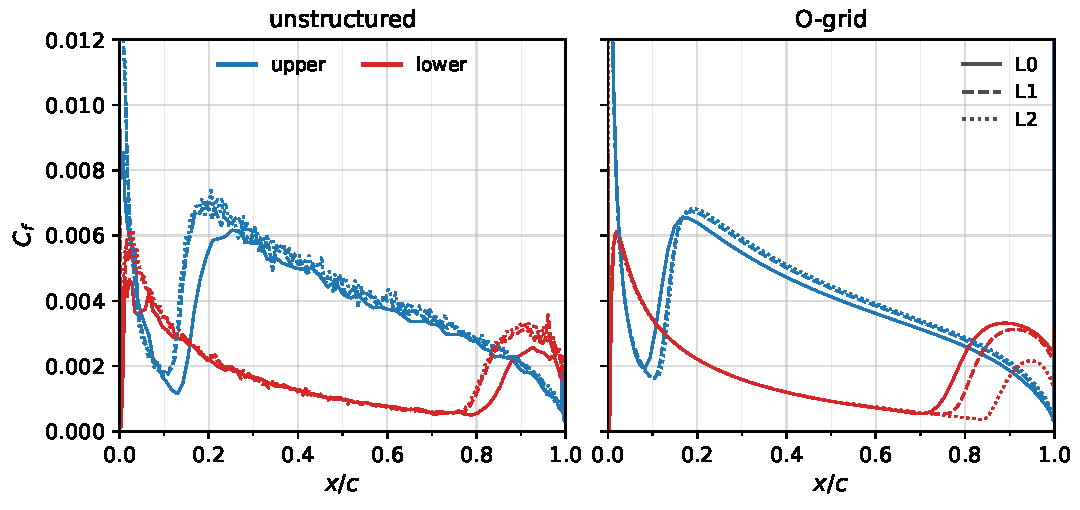
\includegraphics[width=0.95\textwidth]{cf_grid_convergence.pdf}
  \caption{Skin friction on both surfaces of NACA~0012 at $\alpha=4^\circ$ across
  the L0--L2 refinement series (color: upper vs.\ lower surface; line style:
  L0 solid, L1 dashed, L2 dotted), with the two mesh families plotted in separate
  panels to isolate each family's grid convergence from cross-family discrepancies.
  \emph{Left:} the unstructured TE-proper meshes ($3.1\!\times\!10^4$,
  $1.1\!\times\!10^5$, $3.9\!\times\!10^5$ nodes); the laminar dip, transition
  location, and post-transition turbulent level all stabilize from L1 onward, with
  the residual small-amplitude oscillation a tangential staggering of the
  node-centered scheme on the triangulated near-wall layers (it does not bias the
  integral). \emph{Right:} the structured O-grid series ($3.2\!\times\!10^4$,
  $1.3\!\times\!10^5$, $5.1\!\times\!10^5$ nodes); the curves collapse smoothly,
  showing only a small remaining shift of the post-transition level between L1 and
  L2. Both surfaces and both mesh families converge to the same transition
  locations to within $\sim\!1\%$ of chord; the cross-family difference in the
  post-transition turbulent $C_f$ is the gradient-stencil effect on anisotropic
  triangular prism layers discussed in Sec.~\ref{sec:gridconv}, not an unconverged
  grid effect.}
  \label{fig:cfgrid}
\end{figure}

SA-AF transitions over a finite chord band as $\sigma_t$ hands production from
amplification to SA. We report this band as the $10\%$--$90\%$ interval of the
upper-surface skin-friction rise, with the midpoint (steepest-$C_f$ location)
nominal. The band is $\approx\!0.05$--$0.1$ chord wide, narrowing toward the
leading edge at high incidence.
Figure~\ref{fig:xtr} compares this band (shaded) and its midpoint against the $e^N$
reference. On the NACA~0012 the SA-AF transition marches forward with
incidence---from $x/c\approx0.5$ at $\alpha=0^\circ$ to near the leading edge at
$\alpha=8^\circ$---tracking the $e^N$ prediction to within a few percent of chord.
On the NLF(1)-0416 the SA-AF transition sits well aft at low incidence
($x/c\approx0.45$ at $\alpha=0^\circ$) and marches forward with lift, reproducing the
extended laminar run---the low-drag bucket---that is the airfoil's design feature, and
tracking the $e^N$ reference to within $\sim\!0.05$ chord on both grids. The
transition location, not just integrated force, follows the $e^N$ reference
across the operating range, while the absolute drag matches only qualitatively. Figure~\ref{fig:cpcfnlf} shows the NLF(1)-0416 surface
distributions at $\alpha=0^\circ$ on both grids: the laminar run and the
transition location agree closely between the two mesh families on this
natural-laminar-flow geometry.

\begin{figure}[tp]
  \centering
  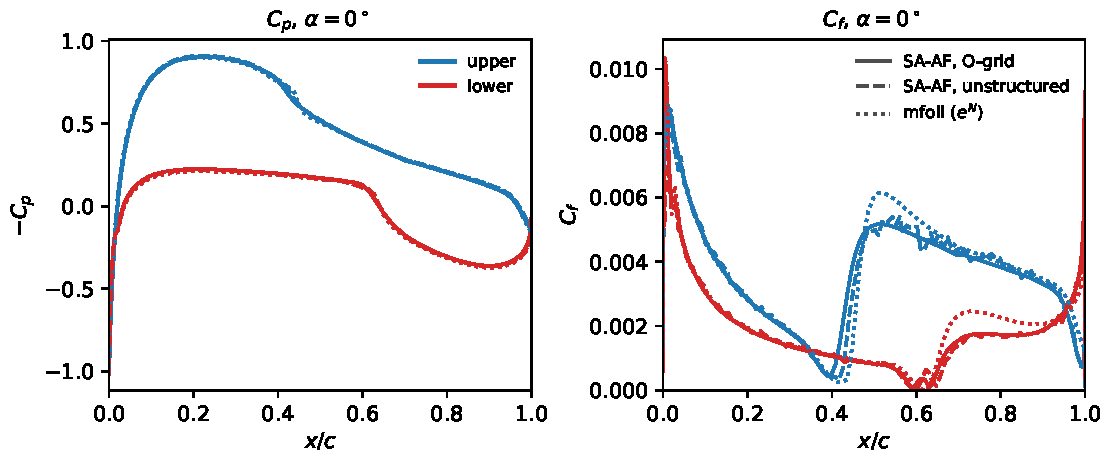
\includegraphics[width=0.95\textwidth]{nlf0416_cp_cf_a0.pdf}
  \caption{NLF(1)-0416 at $\alpha=0^\circ$, both surfaces (color: upper vs.\ lower),
  on a $3.4\!\times\!10^4$-node unstructured and a $5.0\!\times\!10^4$-node O-grid
  (line style: SA-AF O-grid solid, SA-AF unstructured dashed, mfoil $e^N$ dotted).
  The pressure distributions and the long laminar run (transition near $x/c\approx0.45$)
  agree closely between the two grid families and with the $e^N$ reference. (Surfaces are
  separated by walking the airfoil contour and excluding the TE-shared point, rather than
  the sign of the wall-normal coordinate, which on this strongly cambered geometry would
  interleave the upper and lower surfaces over the aft chord.)}
  \label{fig:cpcfnlf}
\end{figure}

\begin{figure}[tp]
  \centering
  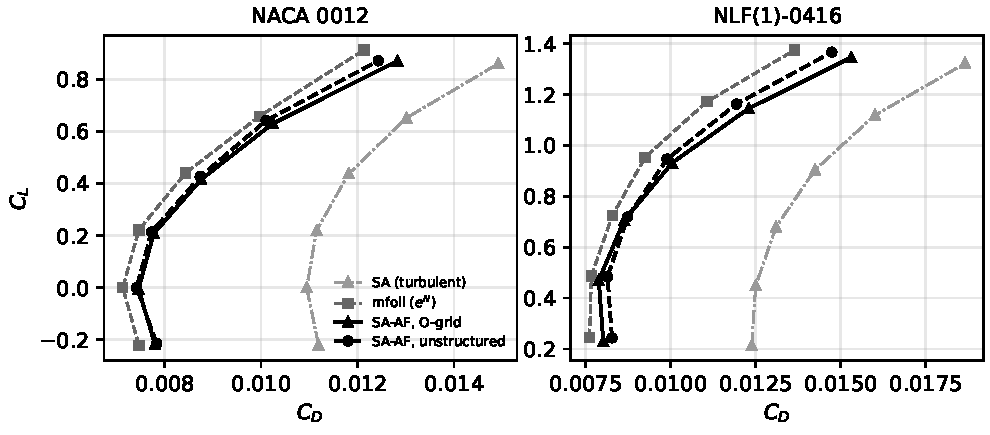
\includegraphics[width=0.95\textwidth]{polar.pdf}
  \caption{Drag polars at $Re=10^6$, $\chi_\infty=0.02$, $\alpha=-2^\circ$ to $8^\circ$,
  on the $\sim\!10^5$-node unstructured (dashed) and $\sim\!10^5$-node O-grid
  (solid) for both airfoils. SA-AF reproduces the $e^N$
  (\texttt{mfoil}) lift--drag relation and the NLF(1)-0416 low-drag bucket on both
  mesh families. The absolute drag is offset high; on the NLF the two grids
  diverge slightly at high incidence (a near-wall/aft-resolution effect, not a
  transition shift).}
  \label{fig:polar}
\end{figure}

\begin{figure}[tp]
  \centering
  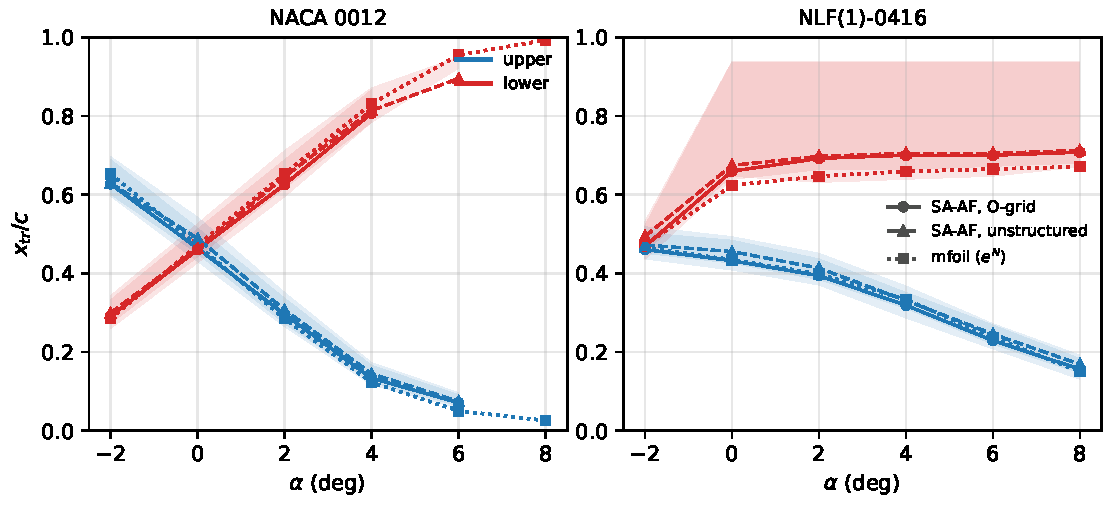
\includegraphics[width=0.95\textwidth]{xtr_alpha.pdf}
  \caption{Transition location vs.\ incidence on both surfaces of NACA~0012
  (left) and NLF(1)-0416 (right) at $Re=10^6$, $\chi_\infty=0.02$. Color
  distinguishes the surface (upper vs.\ lower); line style and marker distinguish
  the solver/grid (SA-AF O-grid: solid line with circle marker; SA-AF
  unstructured: dashed line with triangle marker; mfoil $e^N$ reference: dotted
  line with square marker). Missing data points (e.g.\ NACA~0012 lower surface
  at $\alpha\!=\!8^\circ$) indicate that the rise-detection algorithm found no
  clean laminar-to-turbulent $C_f$ rise in $0.07\le x/c\le0.95$ with
  $C_{f,\mathrm{turb}}/C_{f,\mathrm{lam}}\!\ge\!1.5$; for the NACA~0012 lower
  surface at $\alpha\!=\!8^\circ$ specifically, the boundary layer stays near
  laminar values to the trailing edge.
  Because SA-AF transitions gradually, the SA-AF result is shown as a \emph{band}:
  the shaded region spans the $10\%$--$90\%$ interval of the laminar-to-turbulent
  skin-friction rise; the line marks its midpoint (steepest $C_f$ rise). On both
  airfoils, both surfaces, and both grids, the SA-AF transition tracks the $e^N$
  reference: on the NACA~0012 the upper-surface transition marches forward with
  lift while the lower-surface transition stays aft, and on the NLF(1)-0416 both
  surfaces sit aft at the design incidence ($\alpha\!=\!0^\circ$), recovering the
  low-drag bucket.}
  \label{fig:xtr}
\end{figure}

\section{Conclusion}

The Spalart--Allmaras working variable can serve as its own transition indicator. By
replacing the production in the laminar range with a local, $e^N$-like amplification
rate and reverting to standard SA near $\chi\sim1$, a single transport
equation predicts natural transition without any auxiliary field---occupying a cell
left empty by amplification-factor transport (which transports a separate factor) and
by algebraic SA-transition models (which keep $\tilde\nu$ turbulent and gate it
externally). Because the amplification rate is independent of the working variable,
the modified source keeps an analytic Jacobian and integrates implicitly at the cost
of the baseline model. On a NACA~0012 at zero incidence the model gives a
laminar run and a $\sim\!31\%$ drag reduction, agreeing across the two grids to
$0.5\%$, with the transition mechanism isolated by a same-freestream SA control.

Across an angle-of-attack sweep on two airfoils the predicted transition
tracks an $e^N$ reference and recovers the natural-laminar-flow drag bucket;
the absolute drag matches only qualitatively. Several extensions follow.
Quantitative calibration of the rate against linear-stability and $e^N$
databases beyond the Schubauer--Skramstad anchor used here, and a direct
comparison with the algebraic SA-BCM model on community-standard benchmarks,
would establish accuracy beyond the present demonstration. Extensions to
bypass transition (where the streak-induced mechanism requires a closure that
responds to freestream turbulence energy directly, e.g. the ERCOFTAC T3
series), separation-induced, and crossflow transition are natural next
steps.

\section*{Acknowledgments}
The initial idea for this approach was sparked by conversations with Mark Drela
and Philippe R.\ Spalart, whose insights on the amplification-factor envelope
and on the structure of the SA equation were formative.

\bibliography{references}

\end{document}
